\documentclass[10pt, a4paper]{jsarticle}
\usepackage{amsmath,amssymb}
\usepackage[dvipdfmx]{graphicx}
\usepackage{fancyhdr}
\usepackage{float}
\usepackage{array}
\usepackage{url}

\pagestyle{fancy}
\lhead[\bf \thepage]{\textbf{研究開発リテラシー 最終レポート}} 
\rhead[\bf \thepage]{作成日:\today}
\lfoot{情報工学部 Team RDLG3} 
\cfoot{}
\rfoot{\thepage} 

\title{\LARGE 研究開発リテラシー最終課題\\Webオセロゲーム開発プロジェクト}
\author{Team RDLG3: 吹田暖人,寳中俊介,松井睦玖}
\date{作成日:\today}

\begin{document} 

\maketitle
\tableofcontents

\section{はじめに}\label{sec:introduction}
本レポートでは,研究開発リテラシーの最終課題として開発したWebオセロゲームプロジェクトについて報告する.本プロジェクトは,情報工学部の3名の学生が約2週間にわたって共同開発したWebアプリケーションである.

現代のWeb開発技術を活用し,レスポンシブデザインによるユーザビリティの向上,外部API(Supabase Auth)を用いた認証機能の実装,GitHub Pagesによる静的サイトのデプロイなど,実践的なWeb開発スキルの習得を目的として制作した.

\section{作成物と分担作業}\label{sec:product_overview}

\subsection{作成物の概要}
本プロジェクトで開発したのは,ブラウザ上で動作するオセロ(リバーシ)ゲームのWebアプリケーションである.主な特徴は以下の通りである:

\begin{itemize}
    \item レスポンシブデザインによるPC・スマートフォン対応
    \item Supabase Authを用いたユーザー認証機能
    \item GitHub Pagesによる静的ホスティング
    \item モダンなUI/UXデザイン
    \item 高速動作とシンプルな操作性
\end{itemize}

\subsection{技術スタック}
本プロジェクトで使用した主要な技術は以下の通りである:

\begin{itemize}
    \item \textbf{HTML5}: ページ構造の構築
    \item \textbf{CSS3}: スタイリング・レスポンシブデザインの実装
    \item \textbf{JavaScript}: ゲームロジック・DOM操作の実装
    \item \textbf{Supabase Auth}: ユーザー認証システム
    \item \textbf{GitHub Pages}: 静的サイトのデプロイ・ホスティング
\end{itemize}

\subsection{作業分担}
本プロジェクトの開発における各メンバーの主要な担当分野を表\ref{tab:work_division}に示す.

\begin{table}[H]
\centering
\caption{開発チームの作業分担}
\label{tab:work_division}
\begin{tabular}{|l|p{8cm}|}
\hline
\textbf{メンバー} & \textbf{担当分野・実装内容} \\
\hline
吹田暖人 & 
\begin{itemize}
\item フロントエンド UI/UXデザイン
\item CSS設計・レスポンシブデザインの実装
\item 各ページのスタイリング統一
\end{itemize} \\
\hline
寳中俊介 & 
\begin{itemize}
\item バックエンド・認証機能の実装
\item Supabase連携・セキュリティ対応
\item プロジェクト全体の構成管理
\end{itemize} \\
\hline
松井睦玖 & 
\begin{itemize}
\item ゲームロジックの実装
\item JavaScript・DOM操作の開発
\item アルゴリズムの設計・最適化
\end{itemize} \\
\hline
\end{tabular}
\end{table}

\section{Webページの概要}\label{sec:web_overview}

\subsection{サイト構成}
開発したWebサイトは,以下の主要ページで構成されている:

\begin{itemize}
    \item \textbf{ホームページ} (index.html): サイトの入り口・プロジェクト紹介
    \item \textbf{ゲーム画面} (othello.html): オセロゲームのメイン画面
    \item \textbf{ログイン画面} (auth/login.html): ユーザー認証機能
    \item \textbf{遊び方説明} (howto.html): ゲームルール・操作方法の説明
    \item \textbf{開発者紹介} (developer.html): 開発チームの紹介
    \item \textbf{パスワードリセット} (auth/reset-password.html): アカウント管理機能
\end{itemize}

\subsection{機能概要}
本Webアプリケーションの主要機能は以下の通りである:

\begin{enumerate}
    \item \textbf{オセロゲーム機能}: 8×8ボードでの対戦型オセロゲーム
    \item \textbf{ユーザー認証}: Supabase Authによるログイン・サインアップ機能
    \item \textbf{レスポンシブ対応}: PC・タブレット・スマートフォンでの最適表示
    \item \textbf{ゲームルール表示}: 初心者向けの分かりやすいルール説明
    \item \textbf{開発者情報}: チームメンバーの紹介とGitHubリンク
\end{enumerate}

\section{サイトマップ}\label{sec:sitemap}

図\ref{fig:sitemap}に本Webアプリケーションのサイト構造を示す.

\begin{figure}[H]
\centering
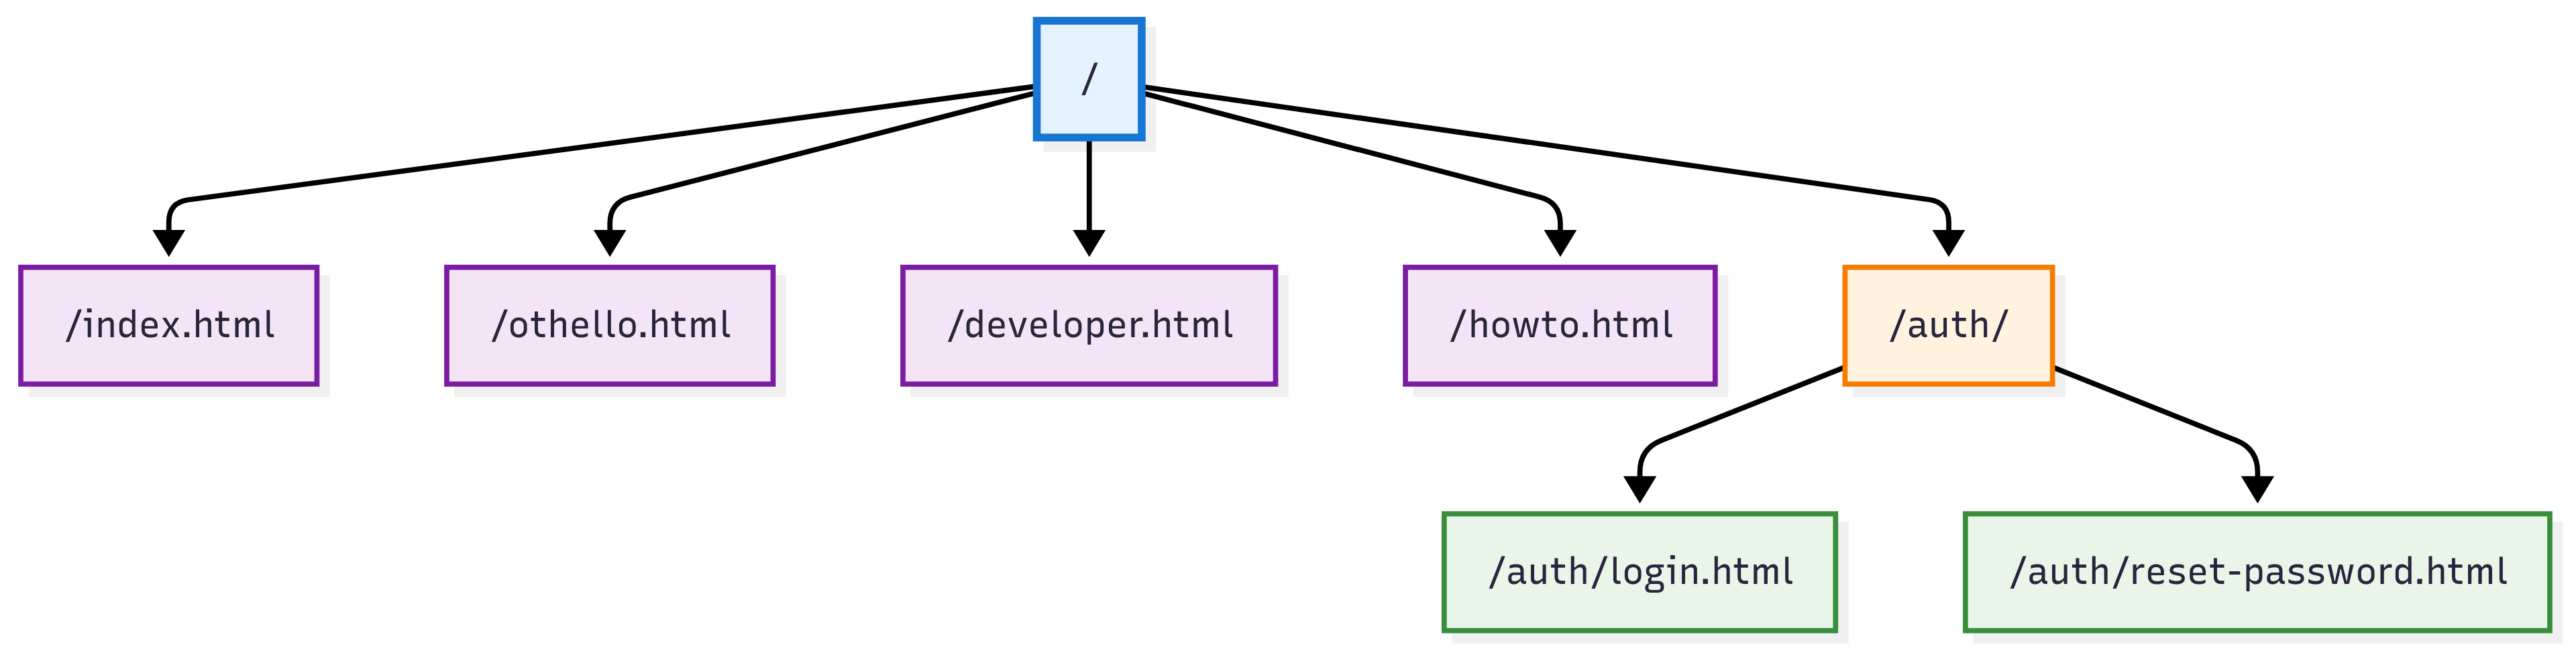
\includegraphics[width=0.8\textwidth]{img/sitemap.png}
\caption{サイトマップ}
\label{fig:sitemap}
\end{figure}

本Webアプリケーションの主要ページ:
\begin{itemize}
    \item \textbf{index.html} (ホームページ) - サイトの入り口
    \item \textbf{othello.html} (ゲーム画面) - オセロゲームのメイン画面
    \item \textbf{developer.html} (開発者紹介) - チームメンバーの紹介
    \item \textbf{howto.html} (遊び方) - ゲームルールの説明
    \item \textbf{auth/login.html} (ログイン) - ユーザー認証
    \item \textbf{auth/reset-password.html} (パスワードリセット) - アカウント管理
\end{itemize}

\section{作業分担}

各メンバーの主要な担当分野:
\begin{itemize}
    \item \textbf{Fukita Hinato}: フロントエンド・UI/UXデザイン
    \item \textbf{Hochu Shunsuke}: バックエンド・認証機能・デプロイ
    \item \textbf{Matsui Riku}: ゲームロジック・JavaScript実装
\end{itemize}

\section{Webページの外観}

本節では,開発したWebページの外観について,PC版とスマートフォン版の画面キャプチャを示す.

\subsection{ホームページ}
図\ref{fig:index-pc}と図\ref{fig:index-phone}にホームページの外観を示す.

\begin{figure}[H]
\centering
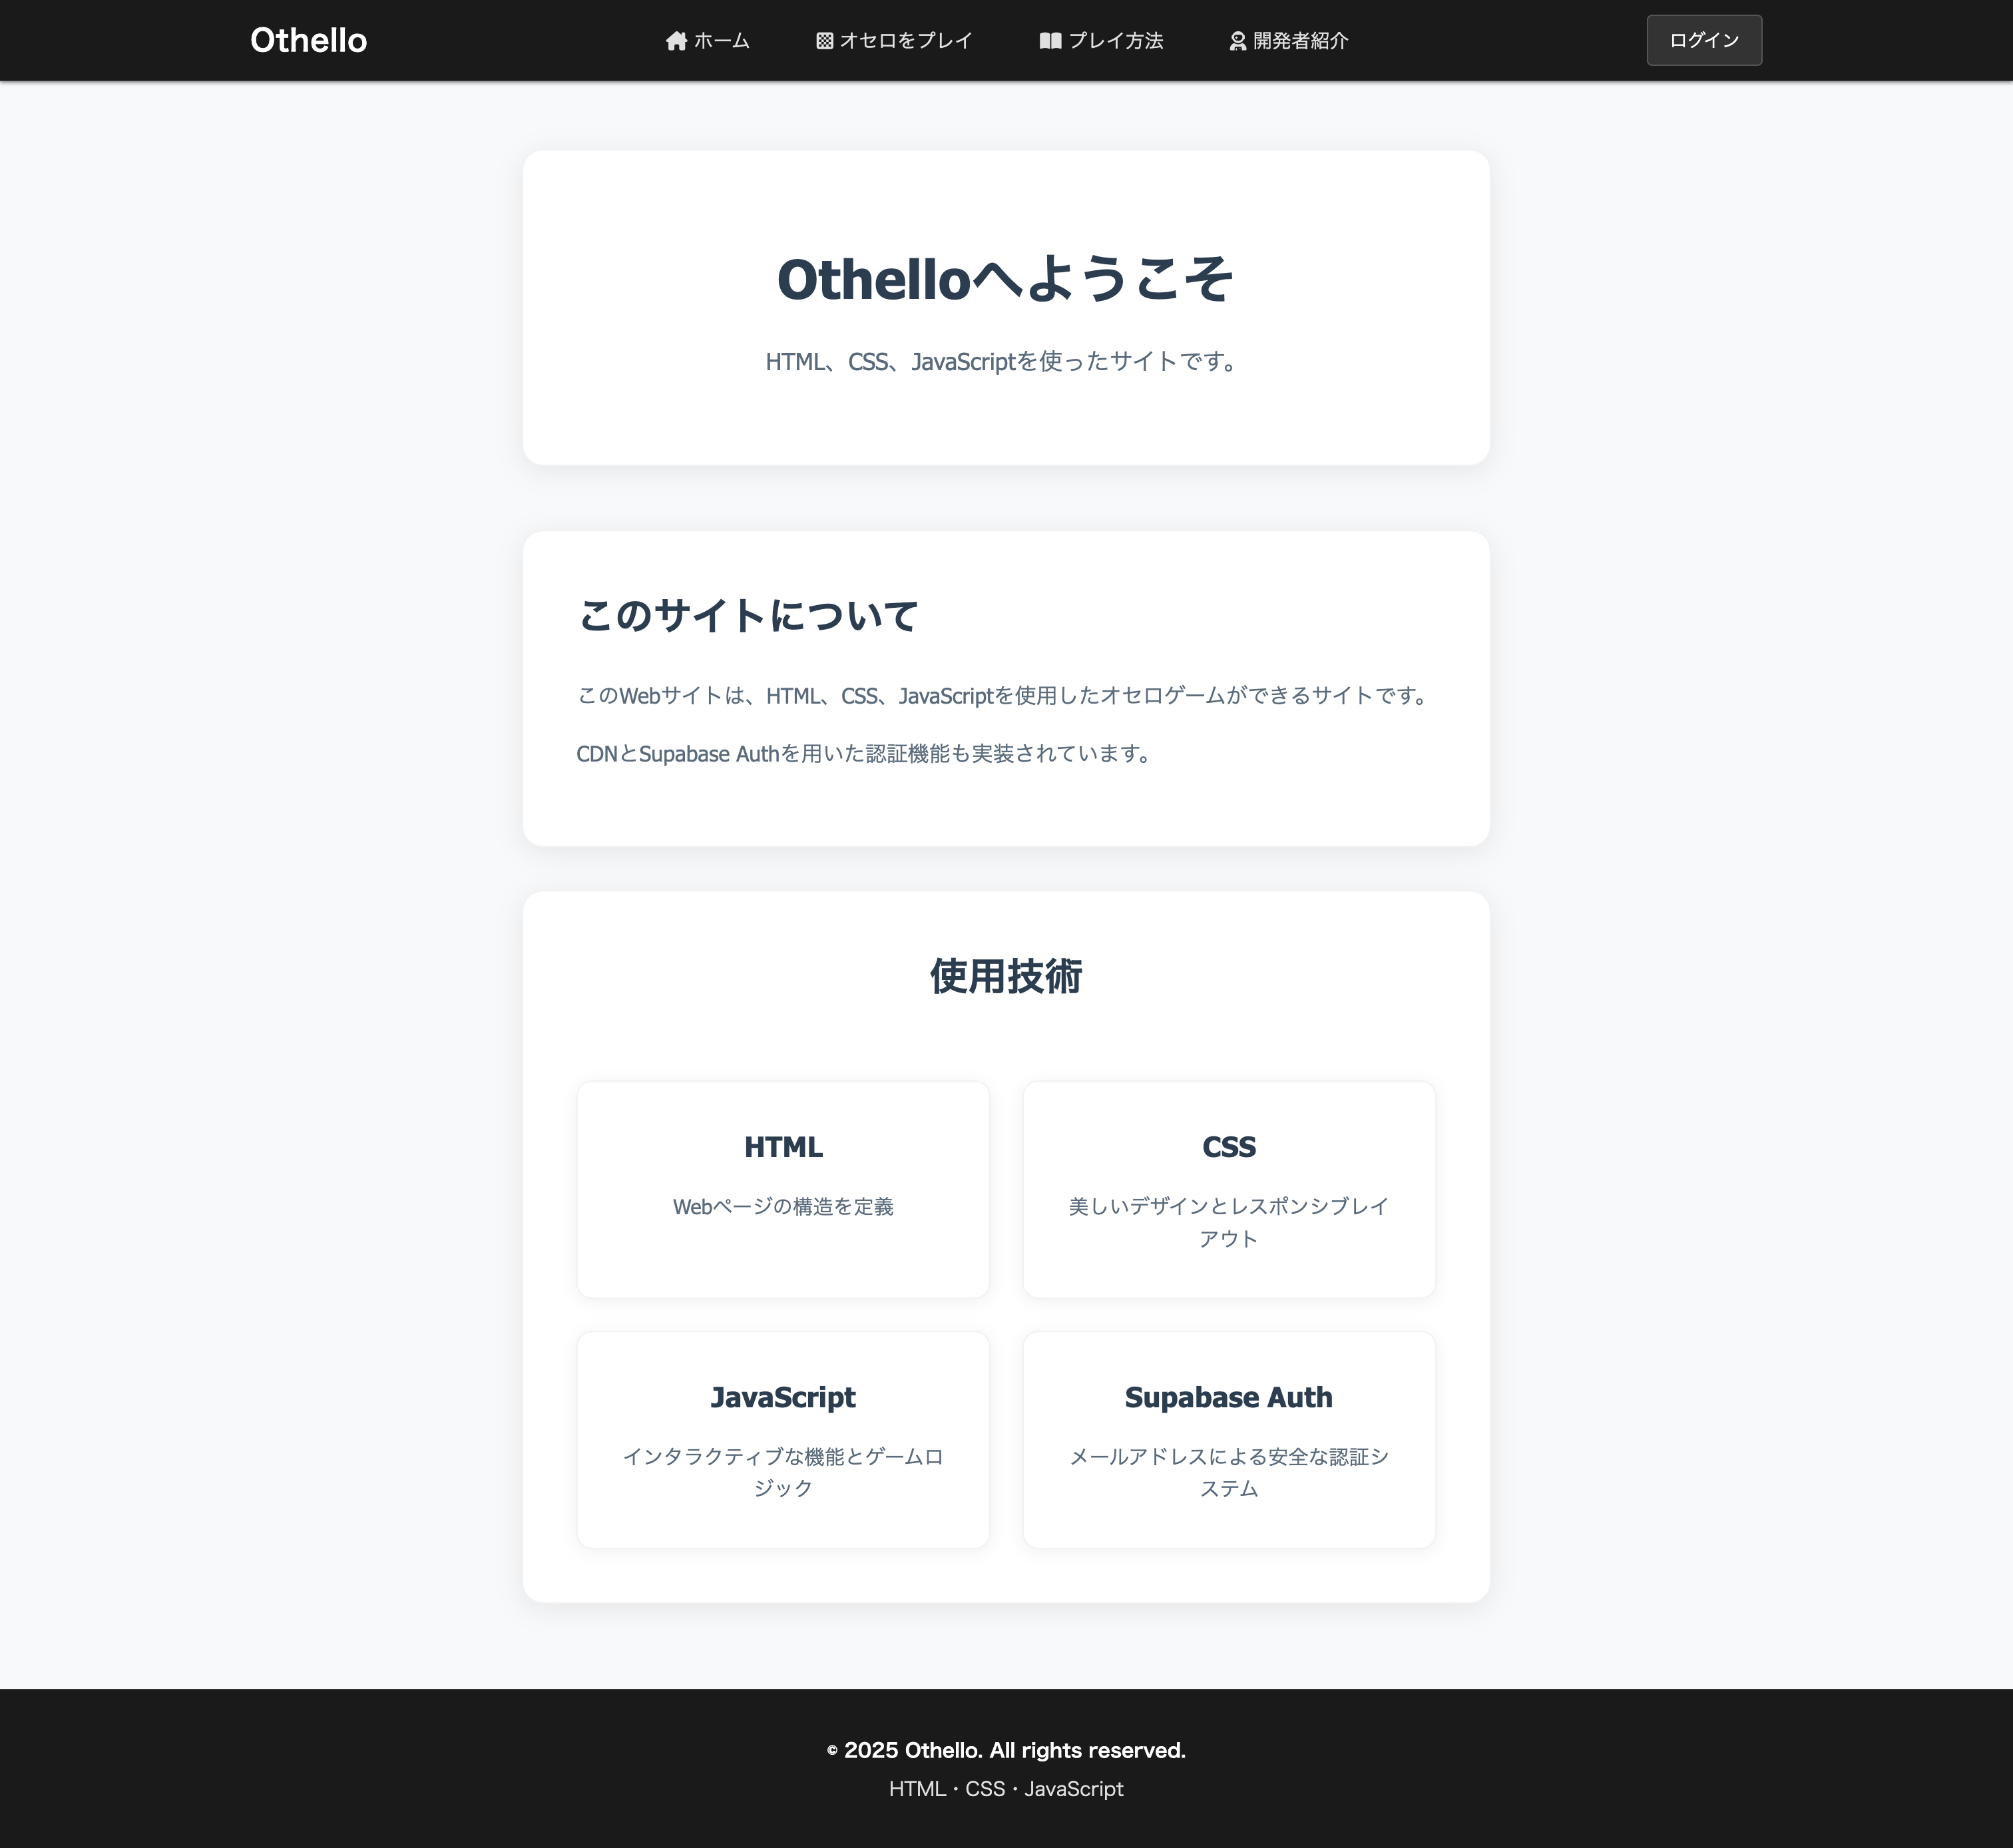
\includegraphics[width=0.7\textwidth]{img/index-pc.png}
\caption{ホームページ(PC版)}
\label{fig:index-pc}
\end{figure}

\begin{figure}[H]
\centering
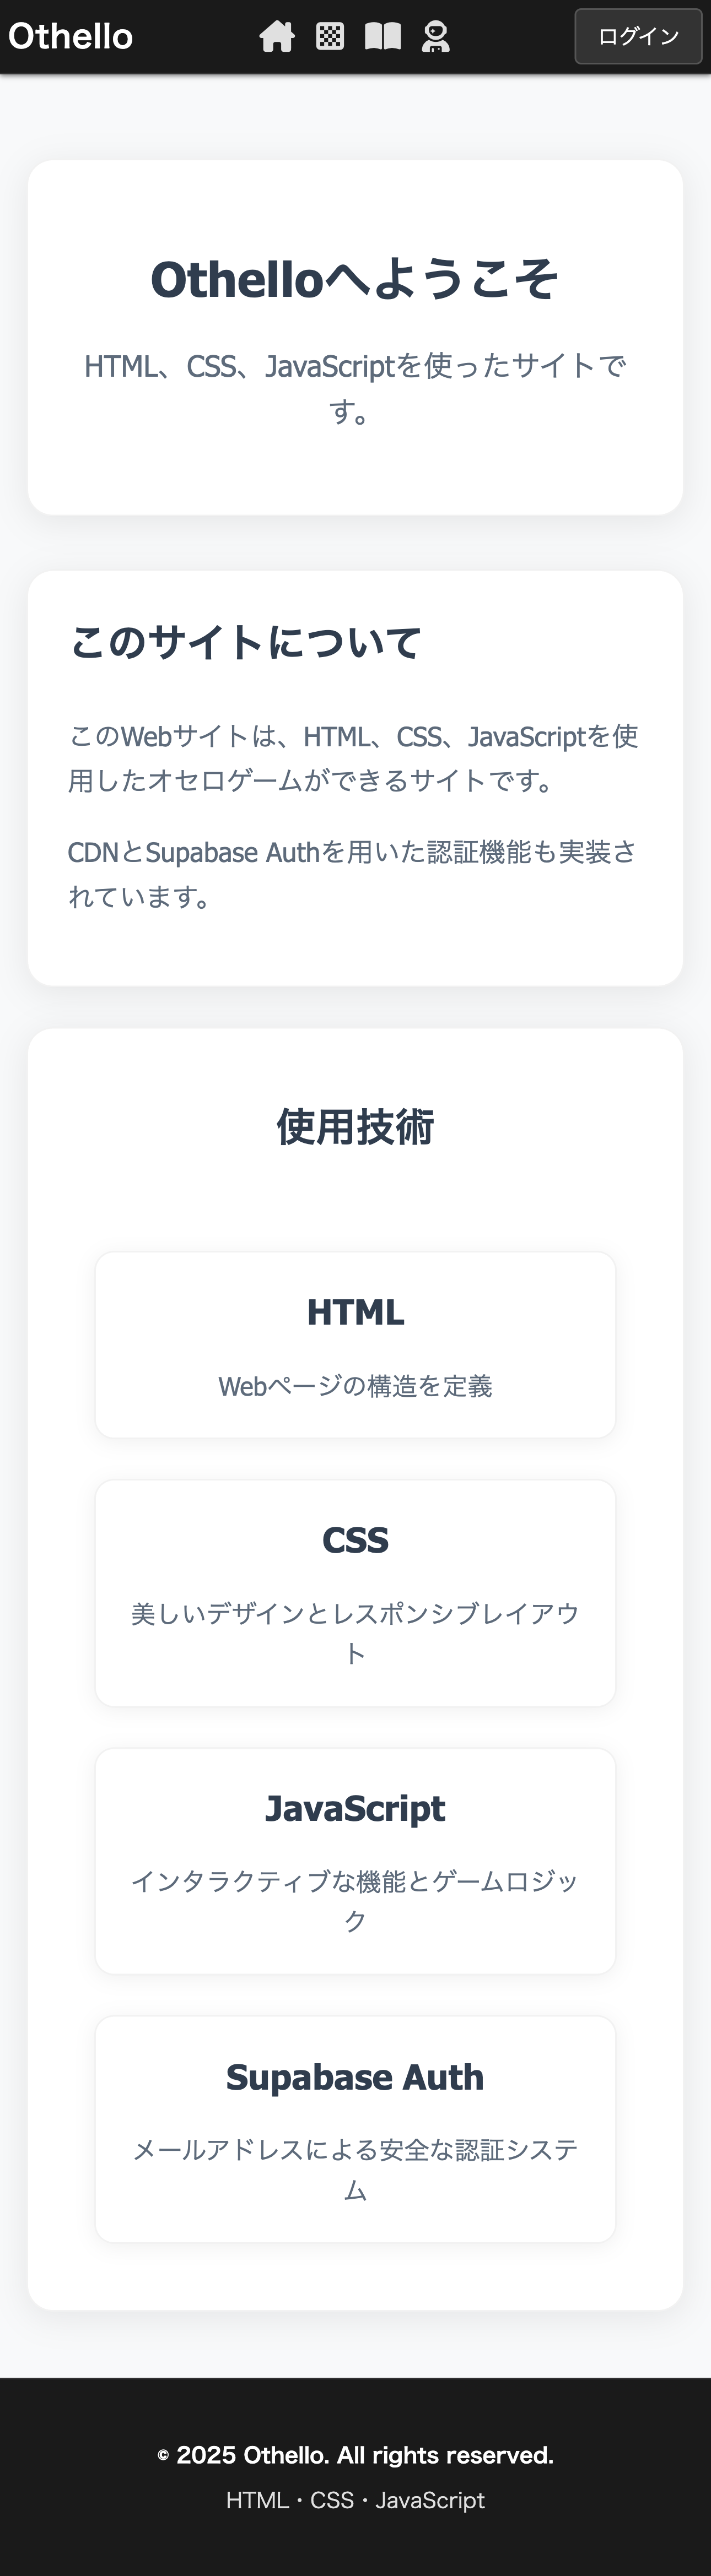
\includegraphics[width=0.4\textwidth]{img/index-phone.png}
\caption{ホームページ(スマートフォン版)}
\label{fig:index-phone}
\end{figure}

\subsection{オセロゲーム画面}
図\ref{fig:othello-pc}と図\ref{fig:othello-phone}にゲームのメイン画面を示す.

\begin{figure}[H]
\centering
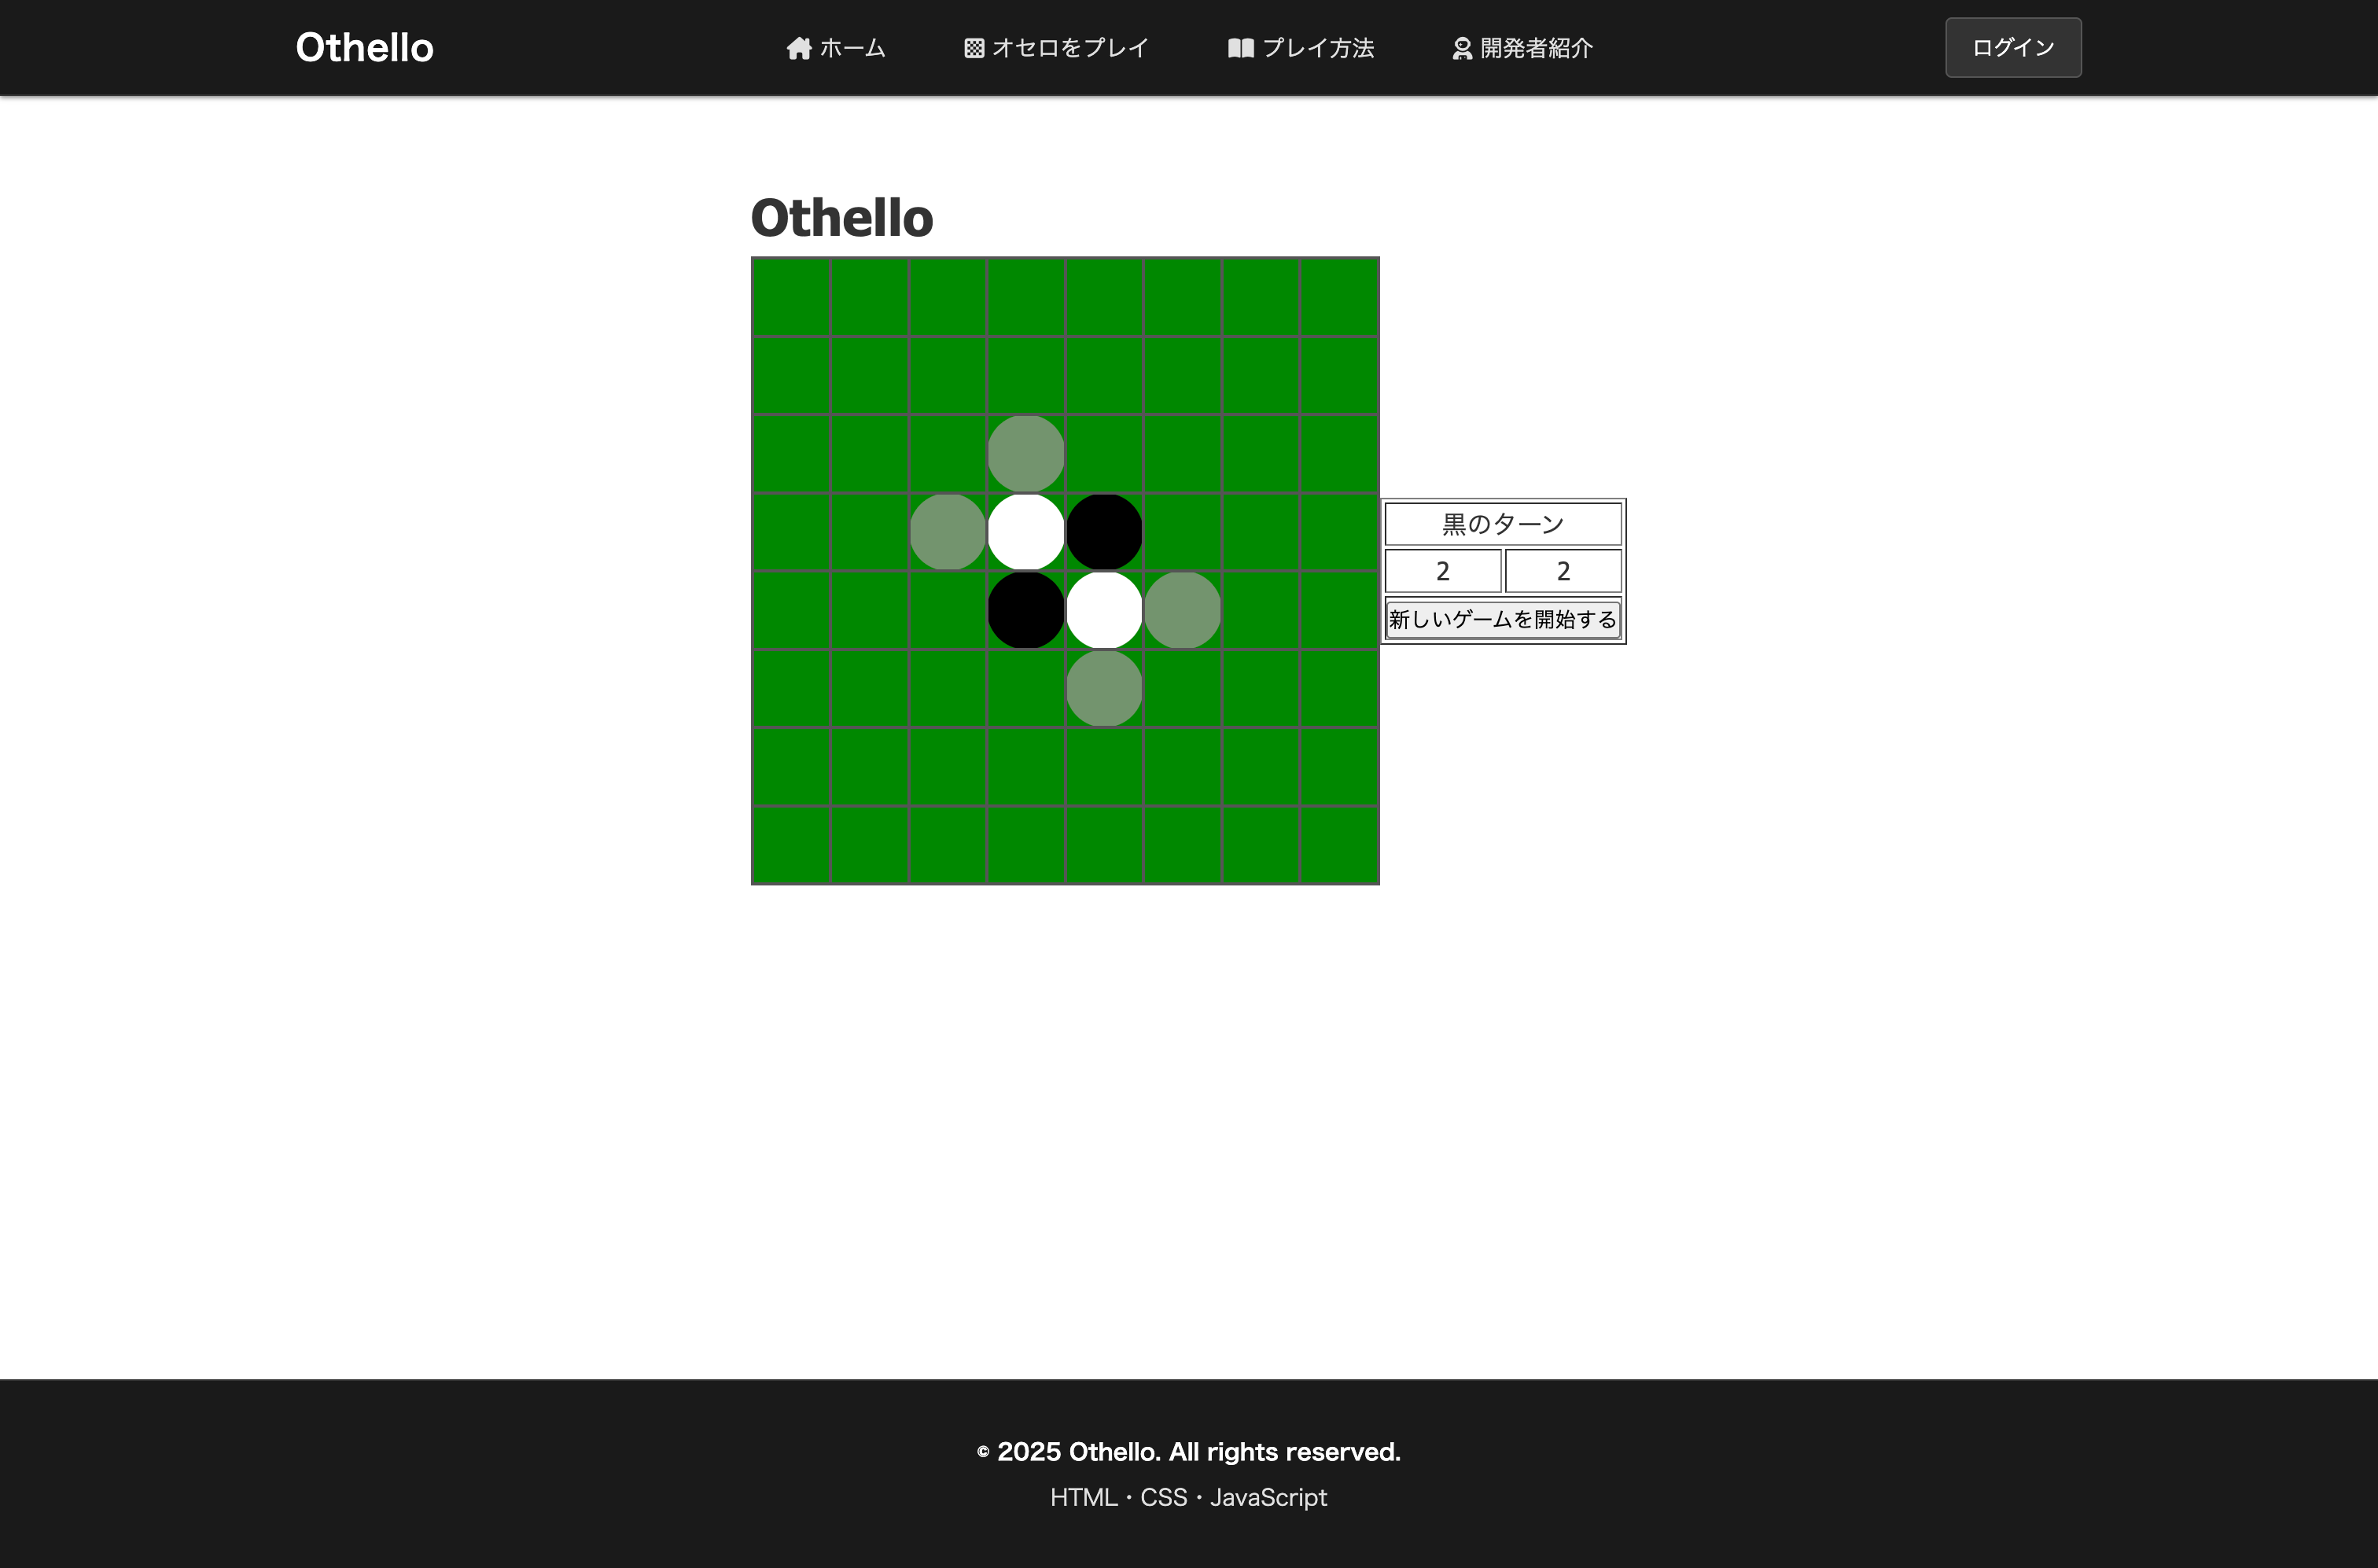
\includegraphics[width=0.7\textwidth]{img/othello-pc.png}
\caption{オセロゲーム画面(PC版)}
\label{fig:othello-pc}
\end{figure}

\begin{figure}[H]
\centering
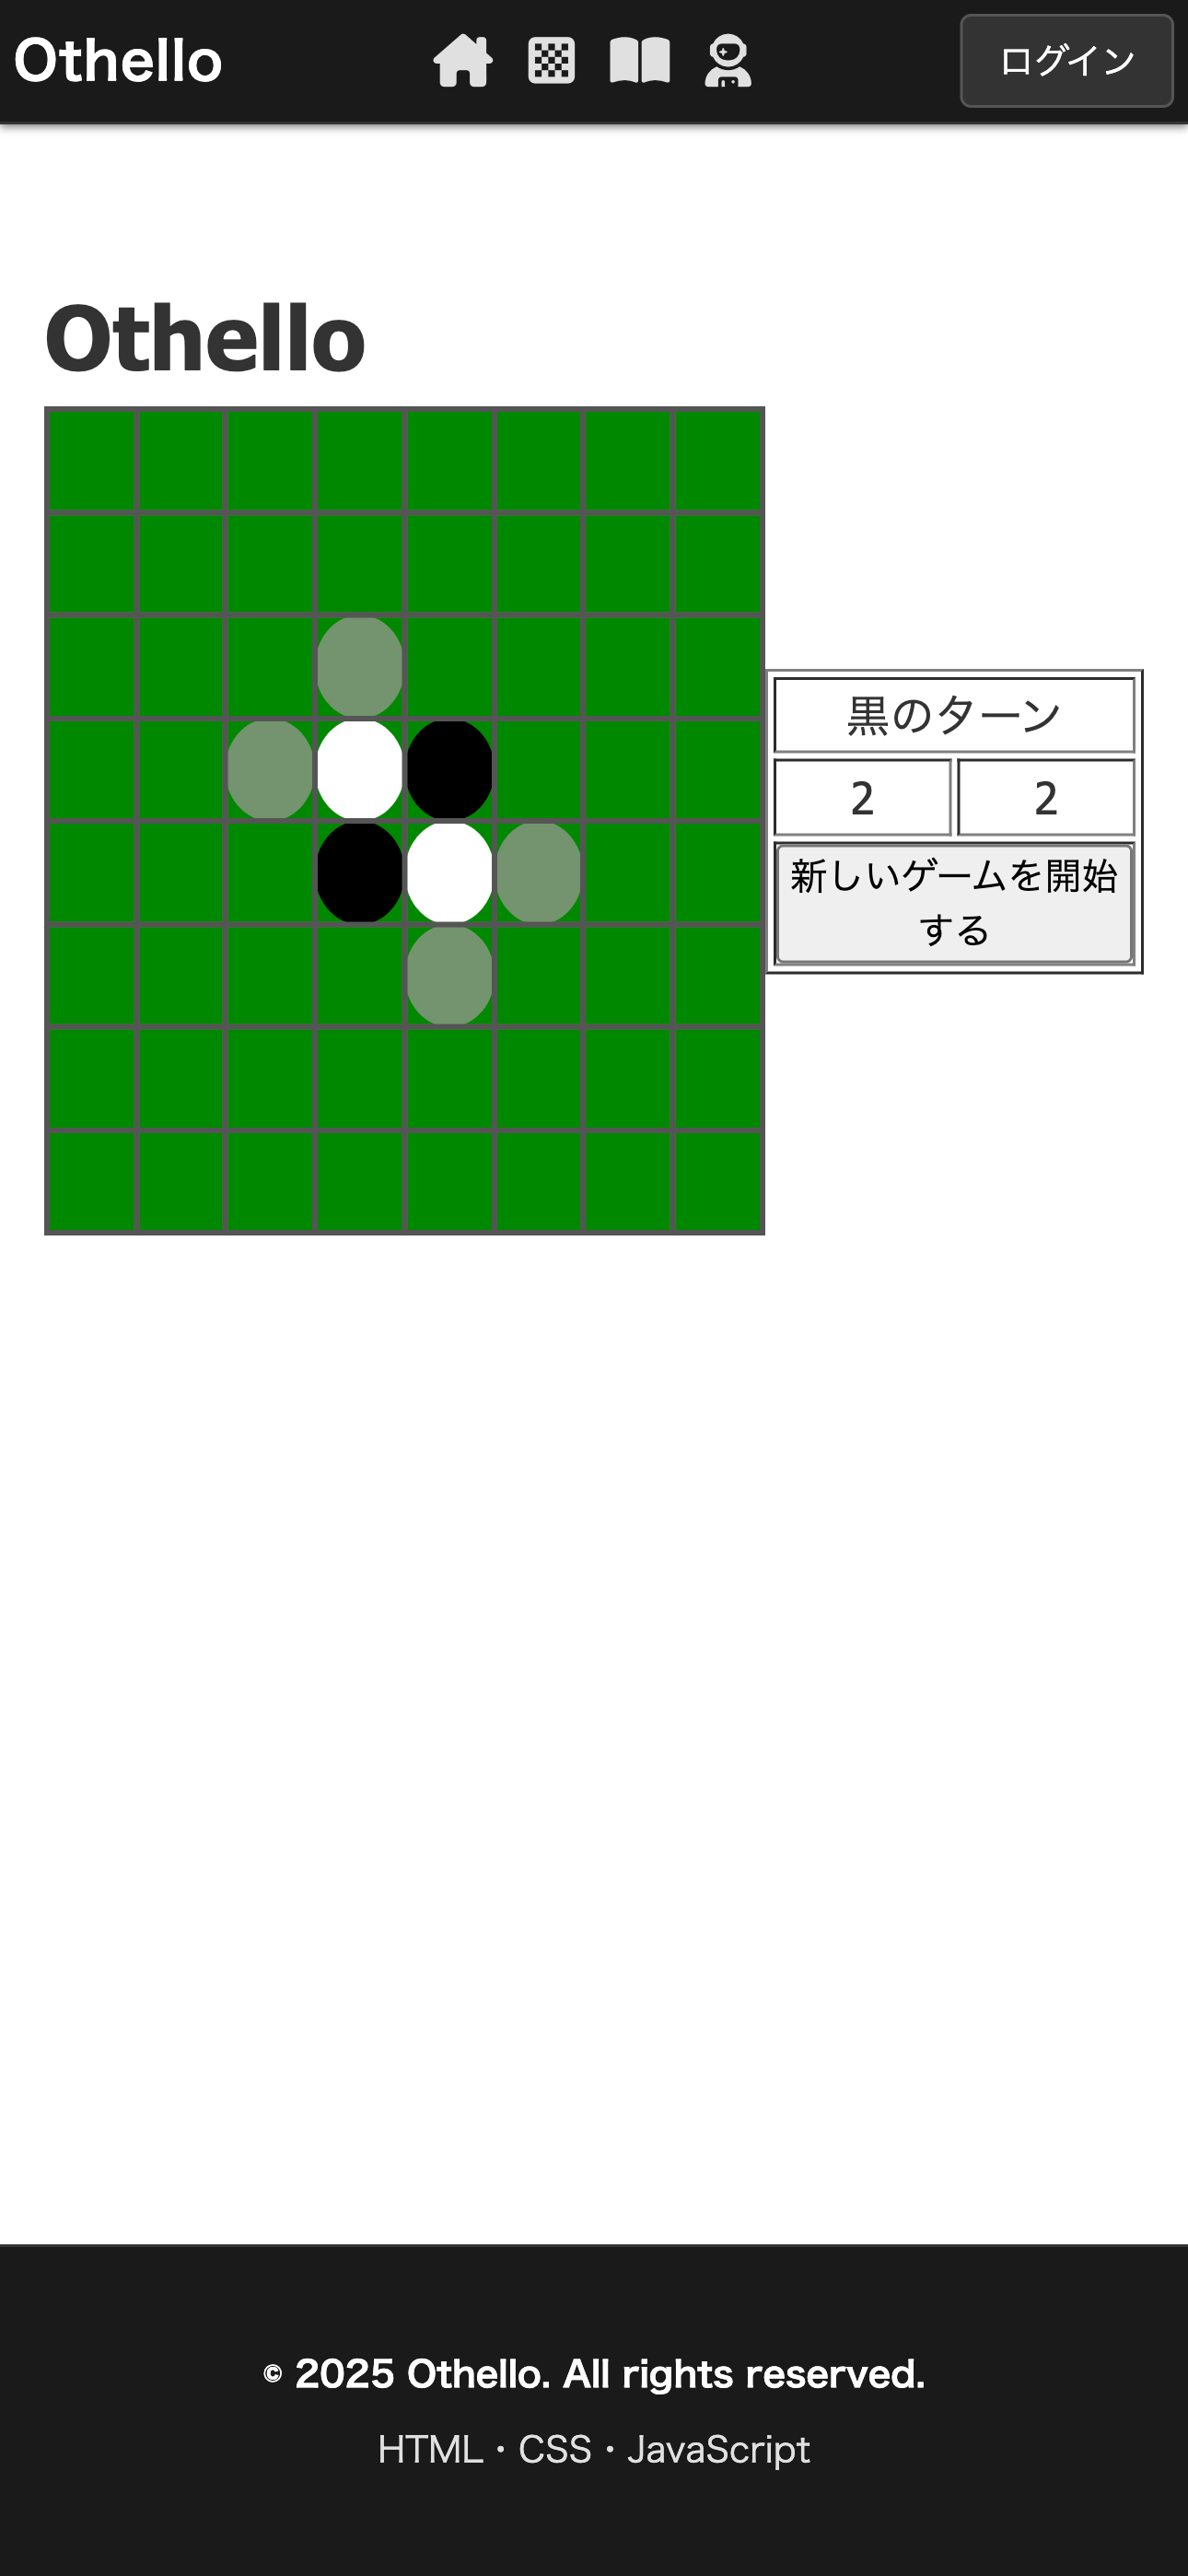
\includegraphics[width=0.4\textwidth]{img/othello-phone.png}
\caption{オセロゲーム画面(スマートフォン版)}
\label{fig:othello-phone}
\end{figure}

\subsection{ログイン画面}
図\ref{fig:login-pc}と図\ref{fig:login-phone}にログイン画面を示す.

\begin{figure}[H]
\centering
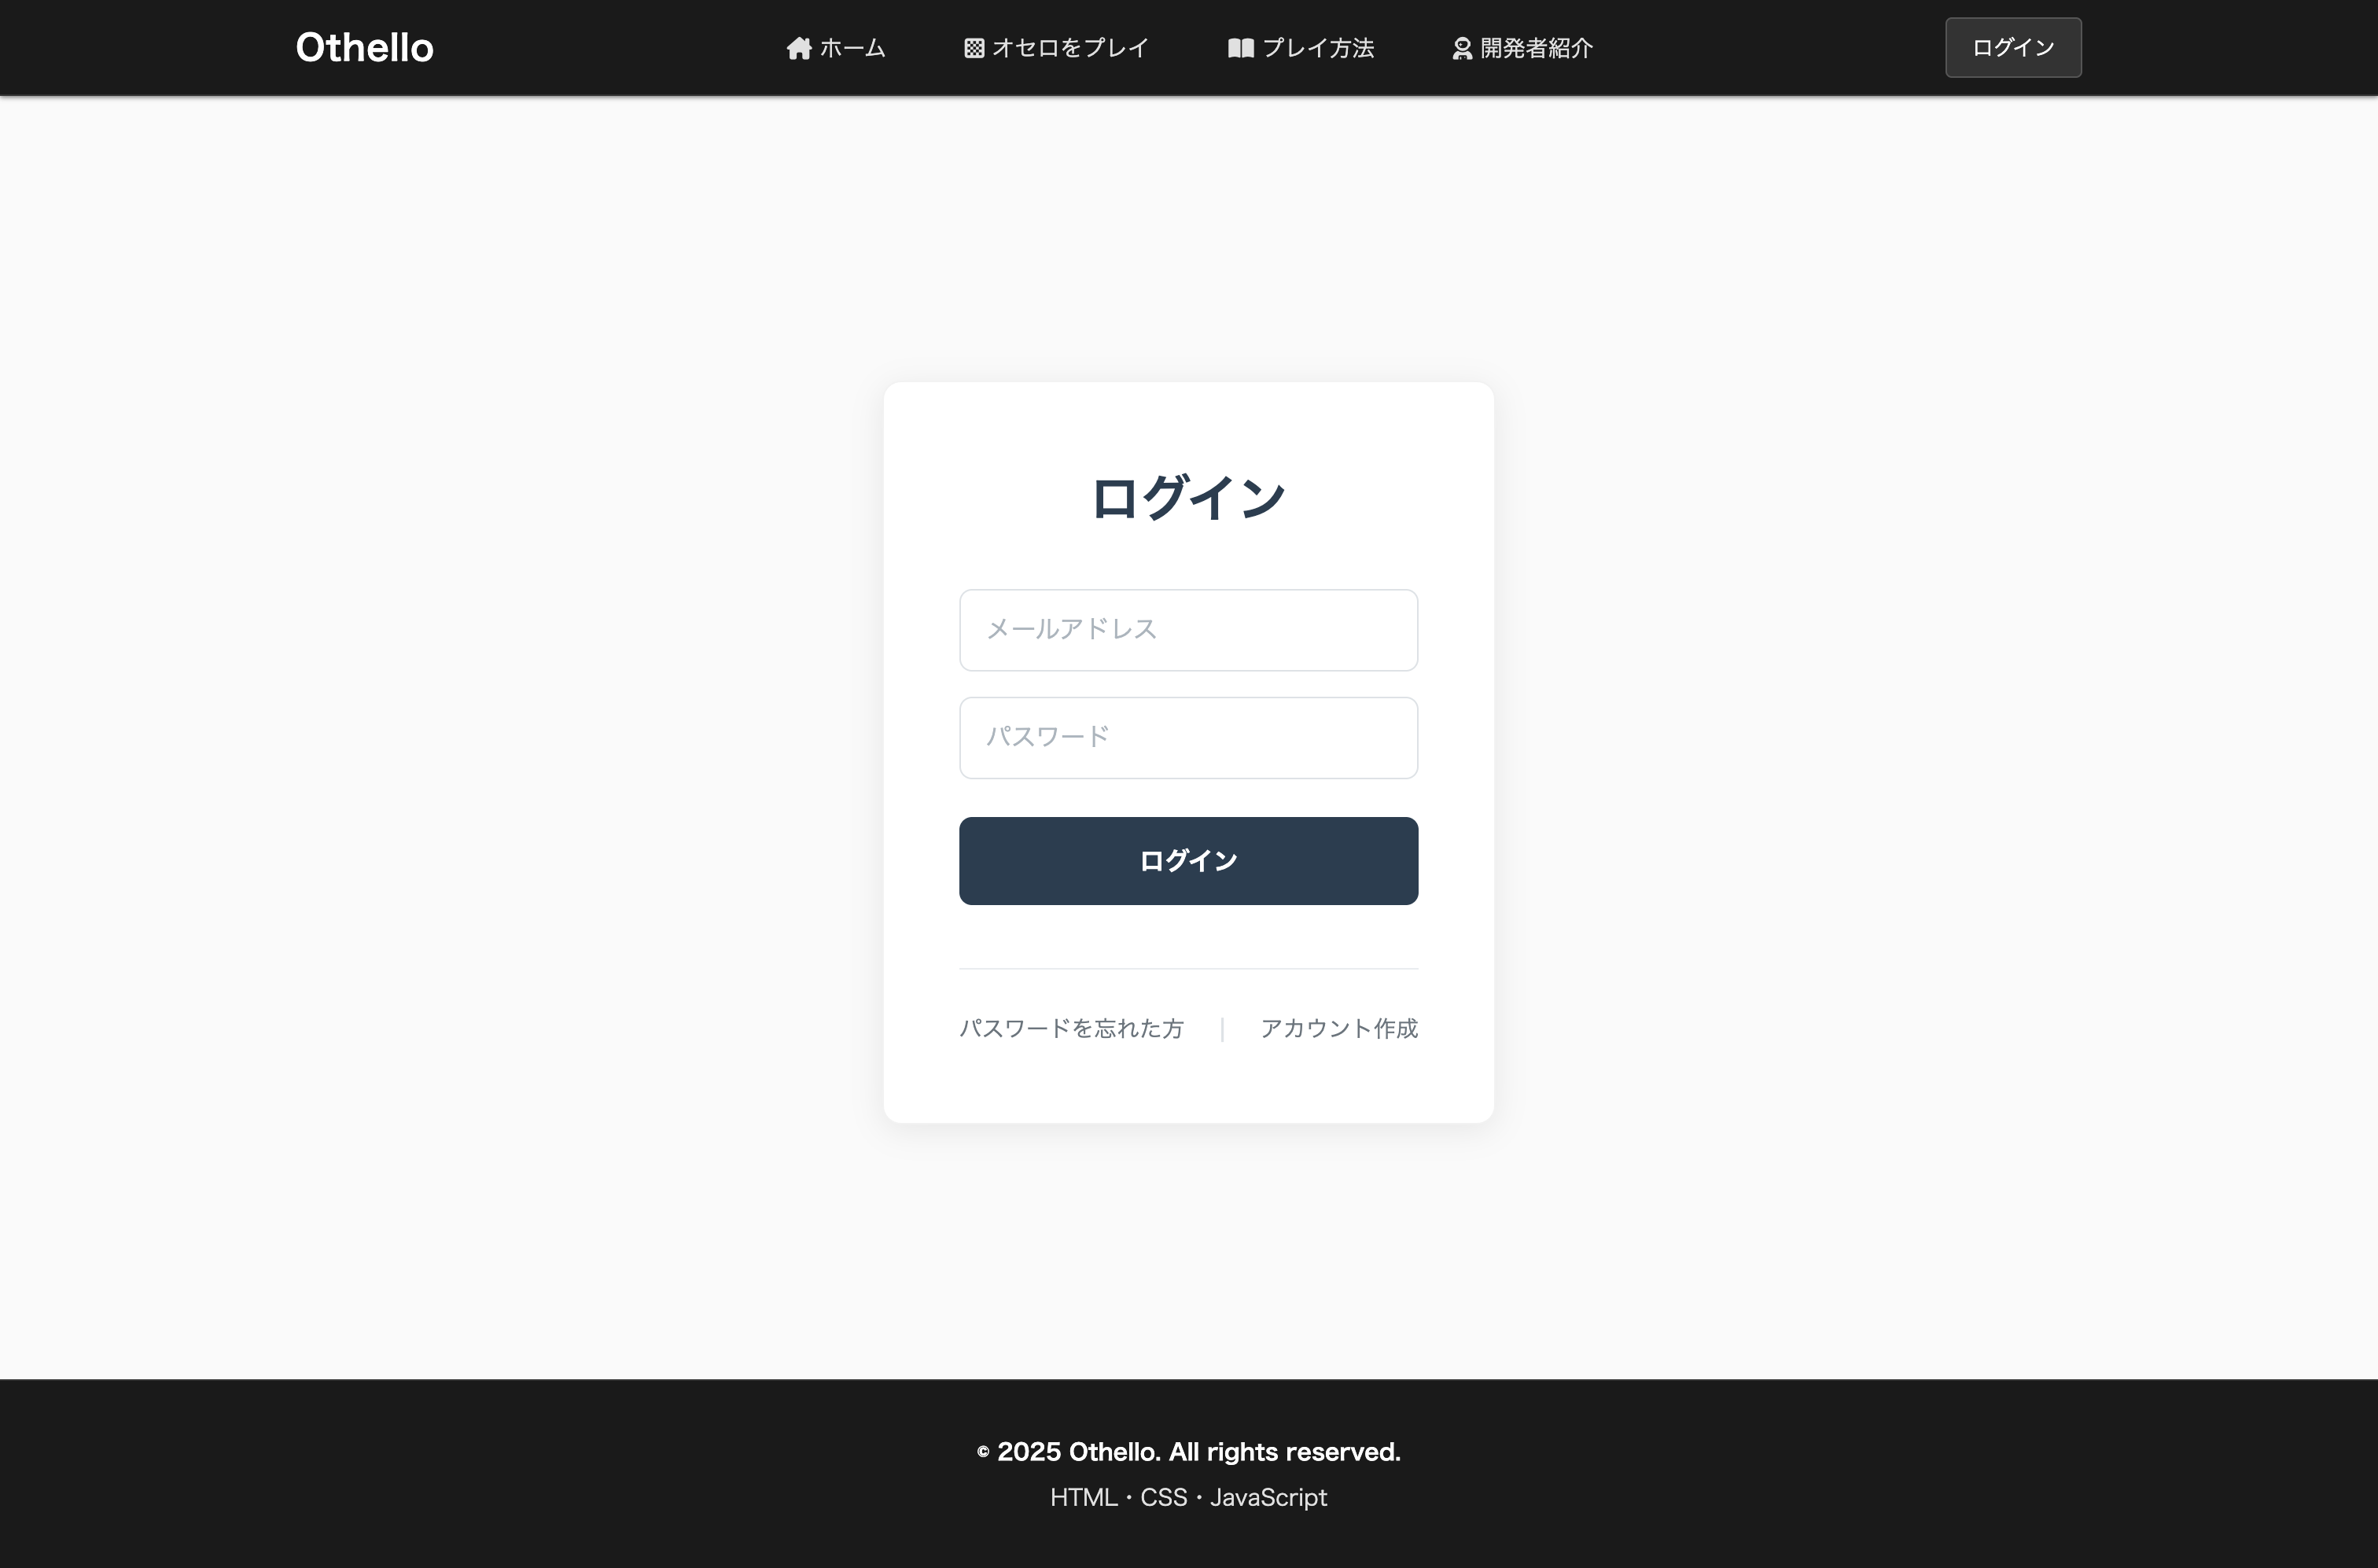
\includegraphics[width=0.7\textwidth]{img/login-pc.png}
\caption{ログイン画面(PC版)}
\label{fig:login-pc}
\end{figure}

\begin{figure}[H]
\centering
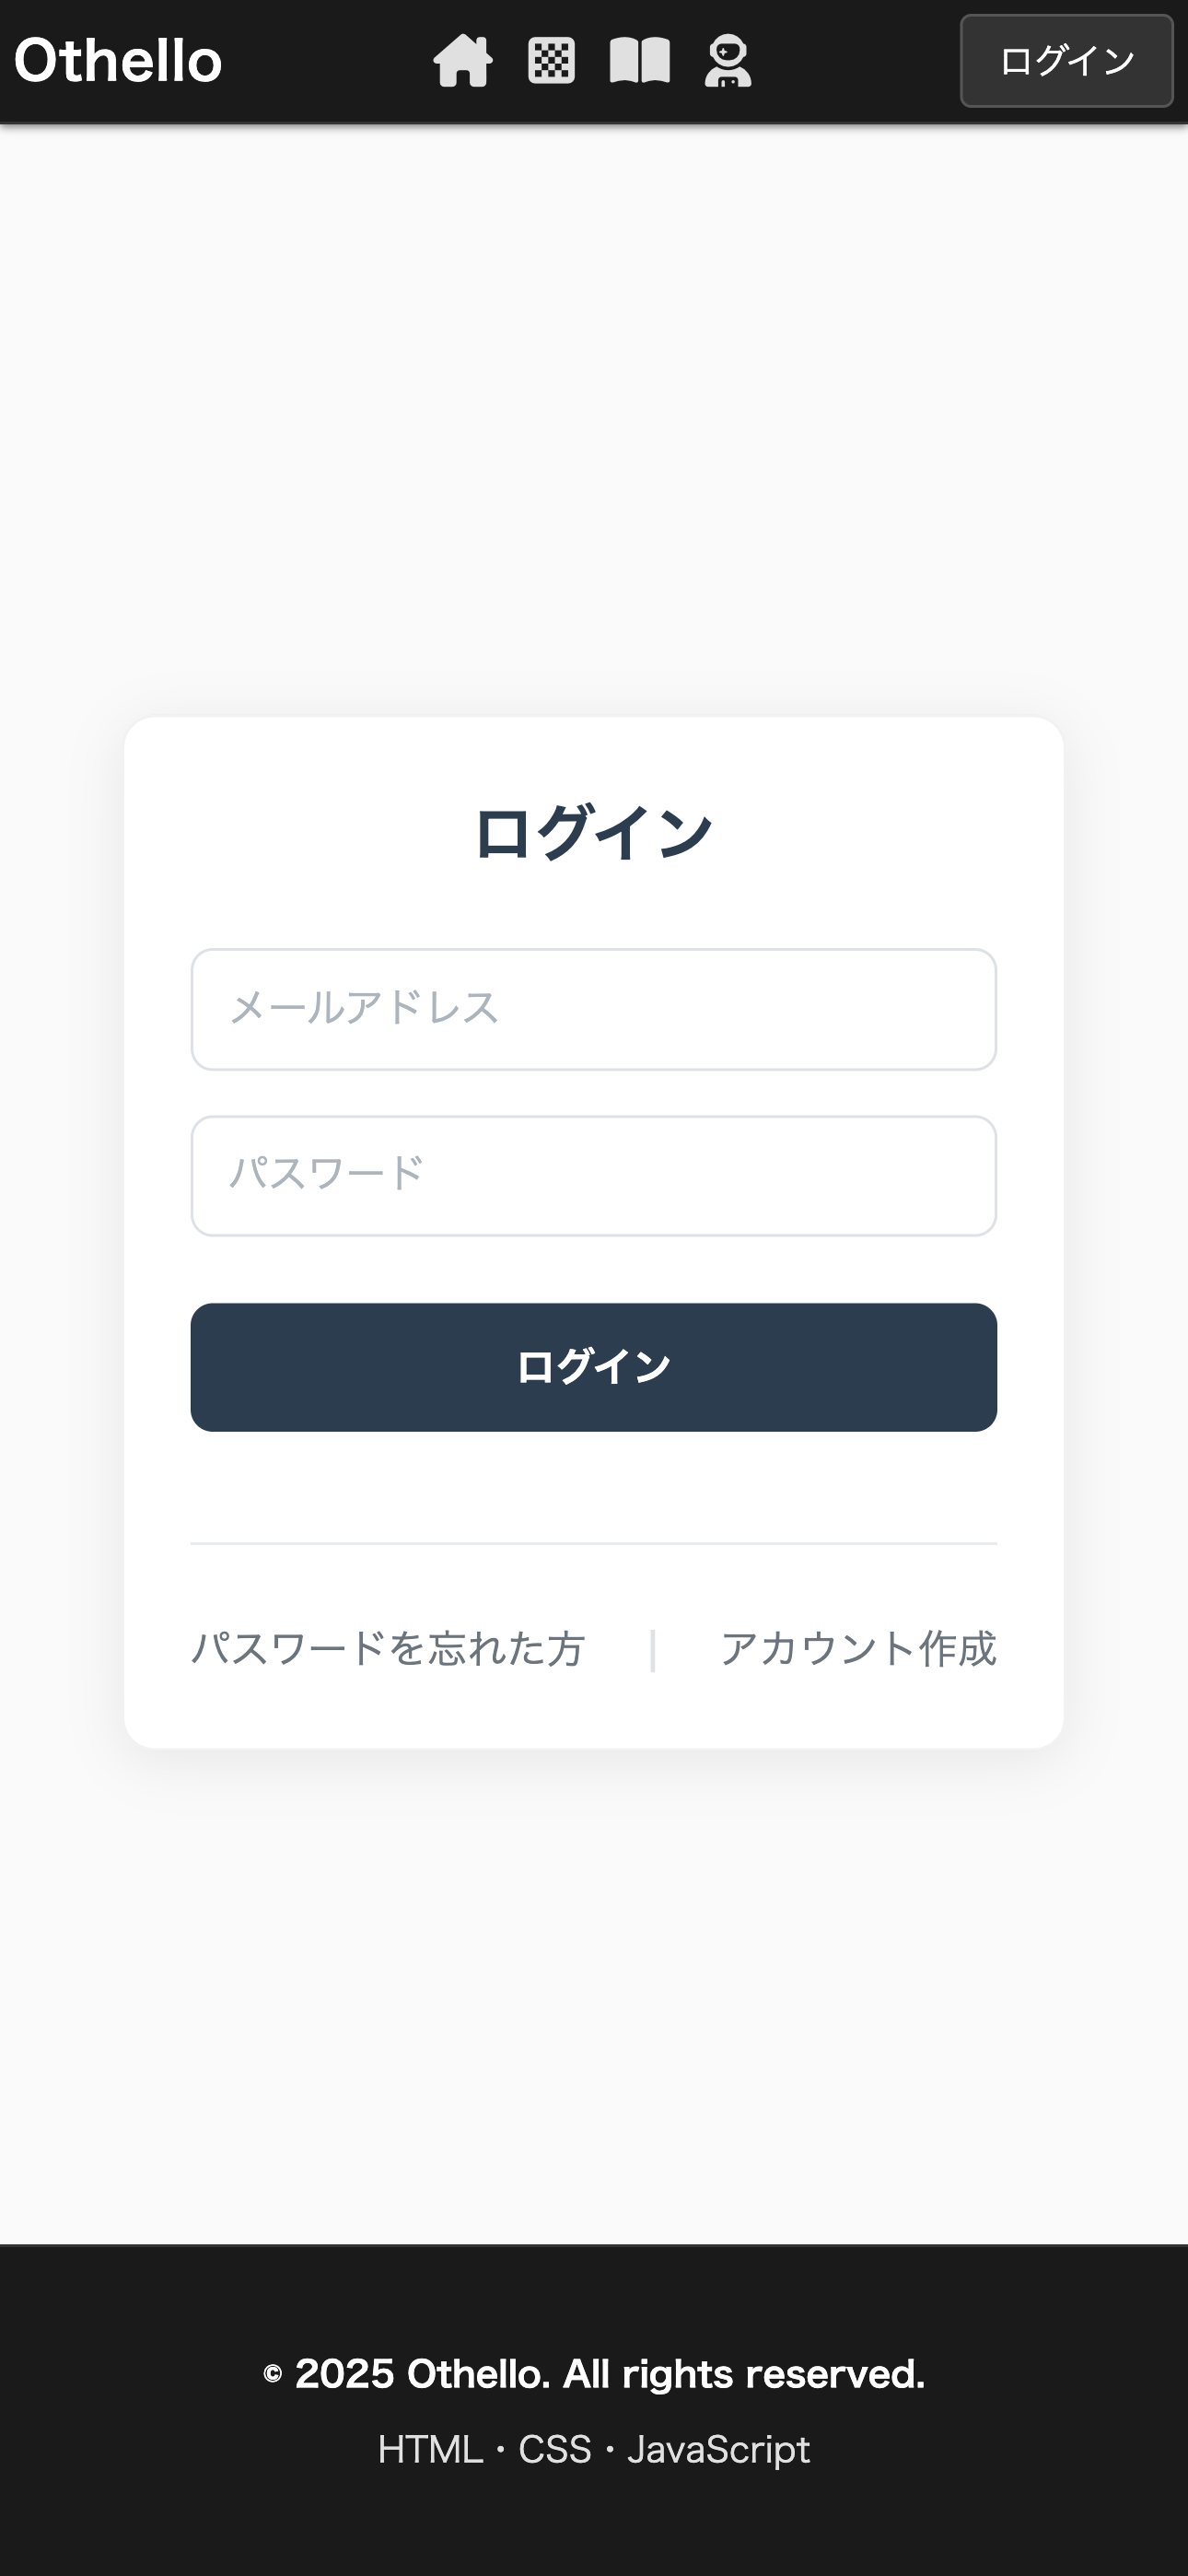
\includegraphics[width=0.4\textwidth]{img/login-phone.png}
\caption{ログイン画面(スマートフォン版)}
\label{fig:login-phone}
\end{figure}

\subsection{サインアップ画面}
図\ref{fig:signup-pc}と図\ref{fig:signup-phone}にサインアップ画面を示す.

\begin{figure}[H]
\centering
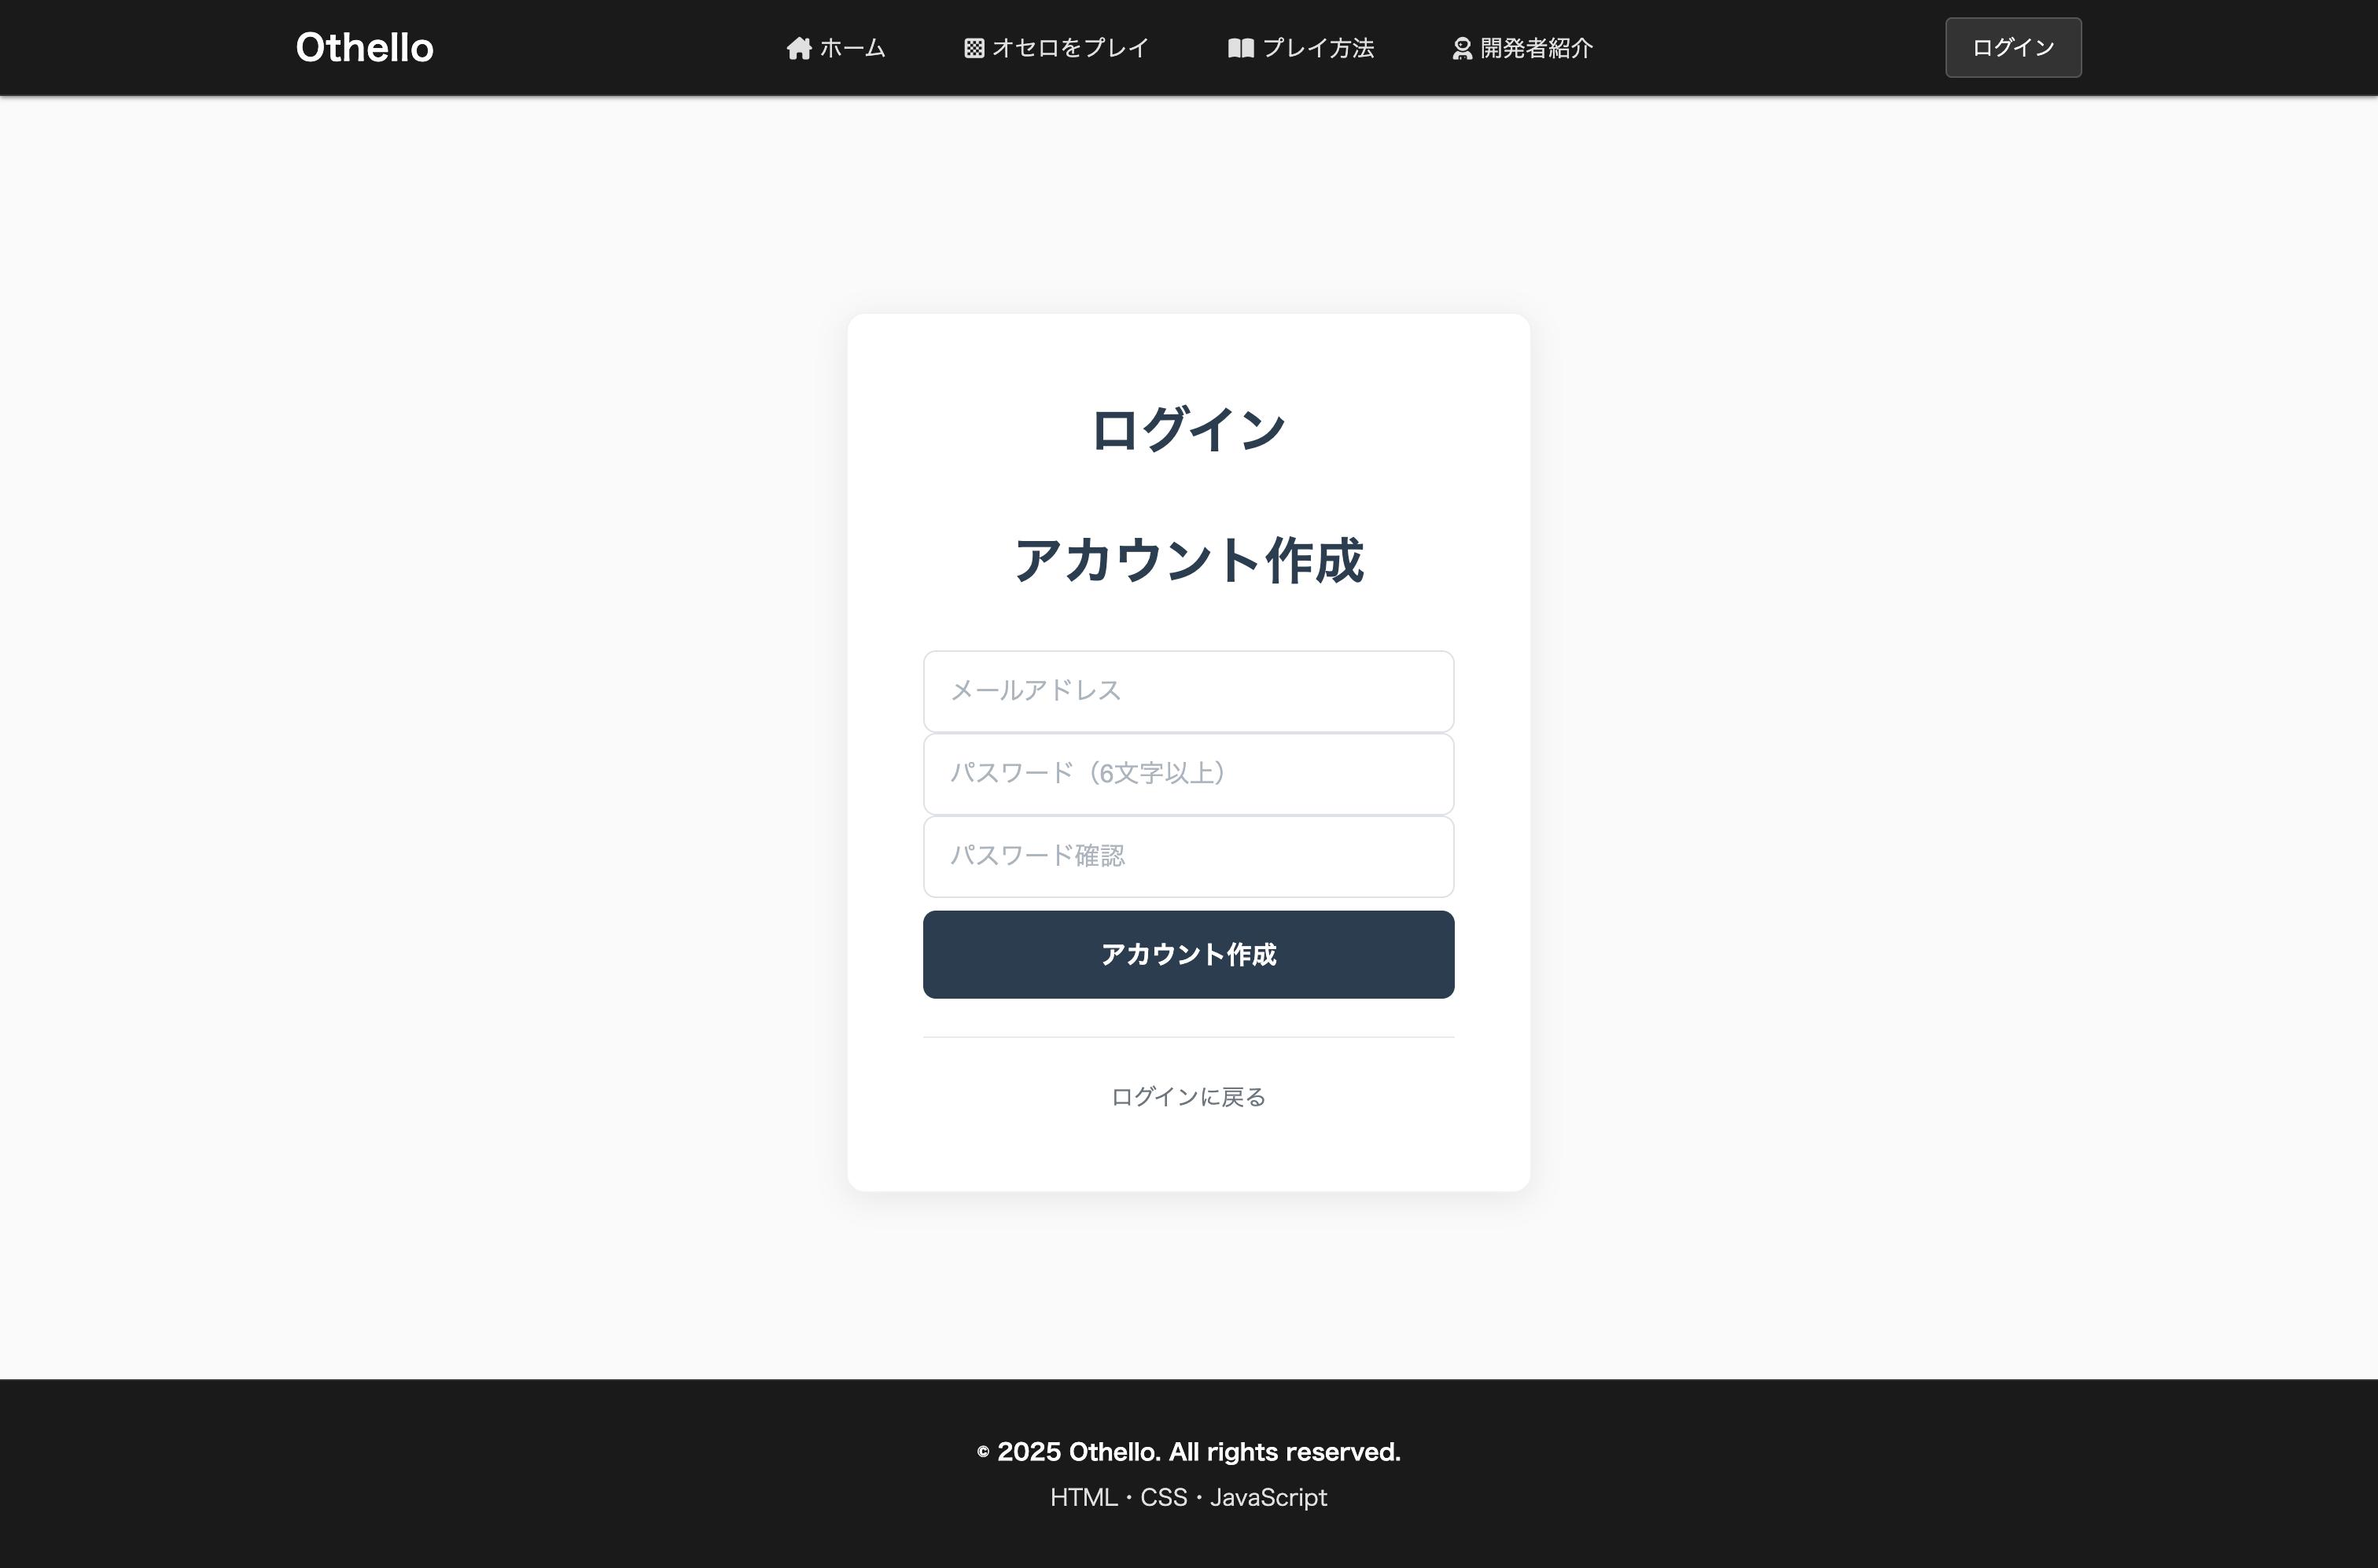
\includegraphics[width=0.7\textwidth]{img/signup-pc.png}
\caption{サインアップ画面(PC版)}
\label{fig:signup-pc}
\end{figure}

\begin{figure}[H]
\centering
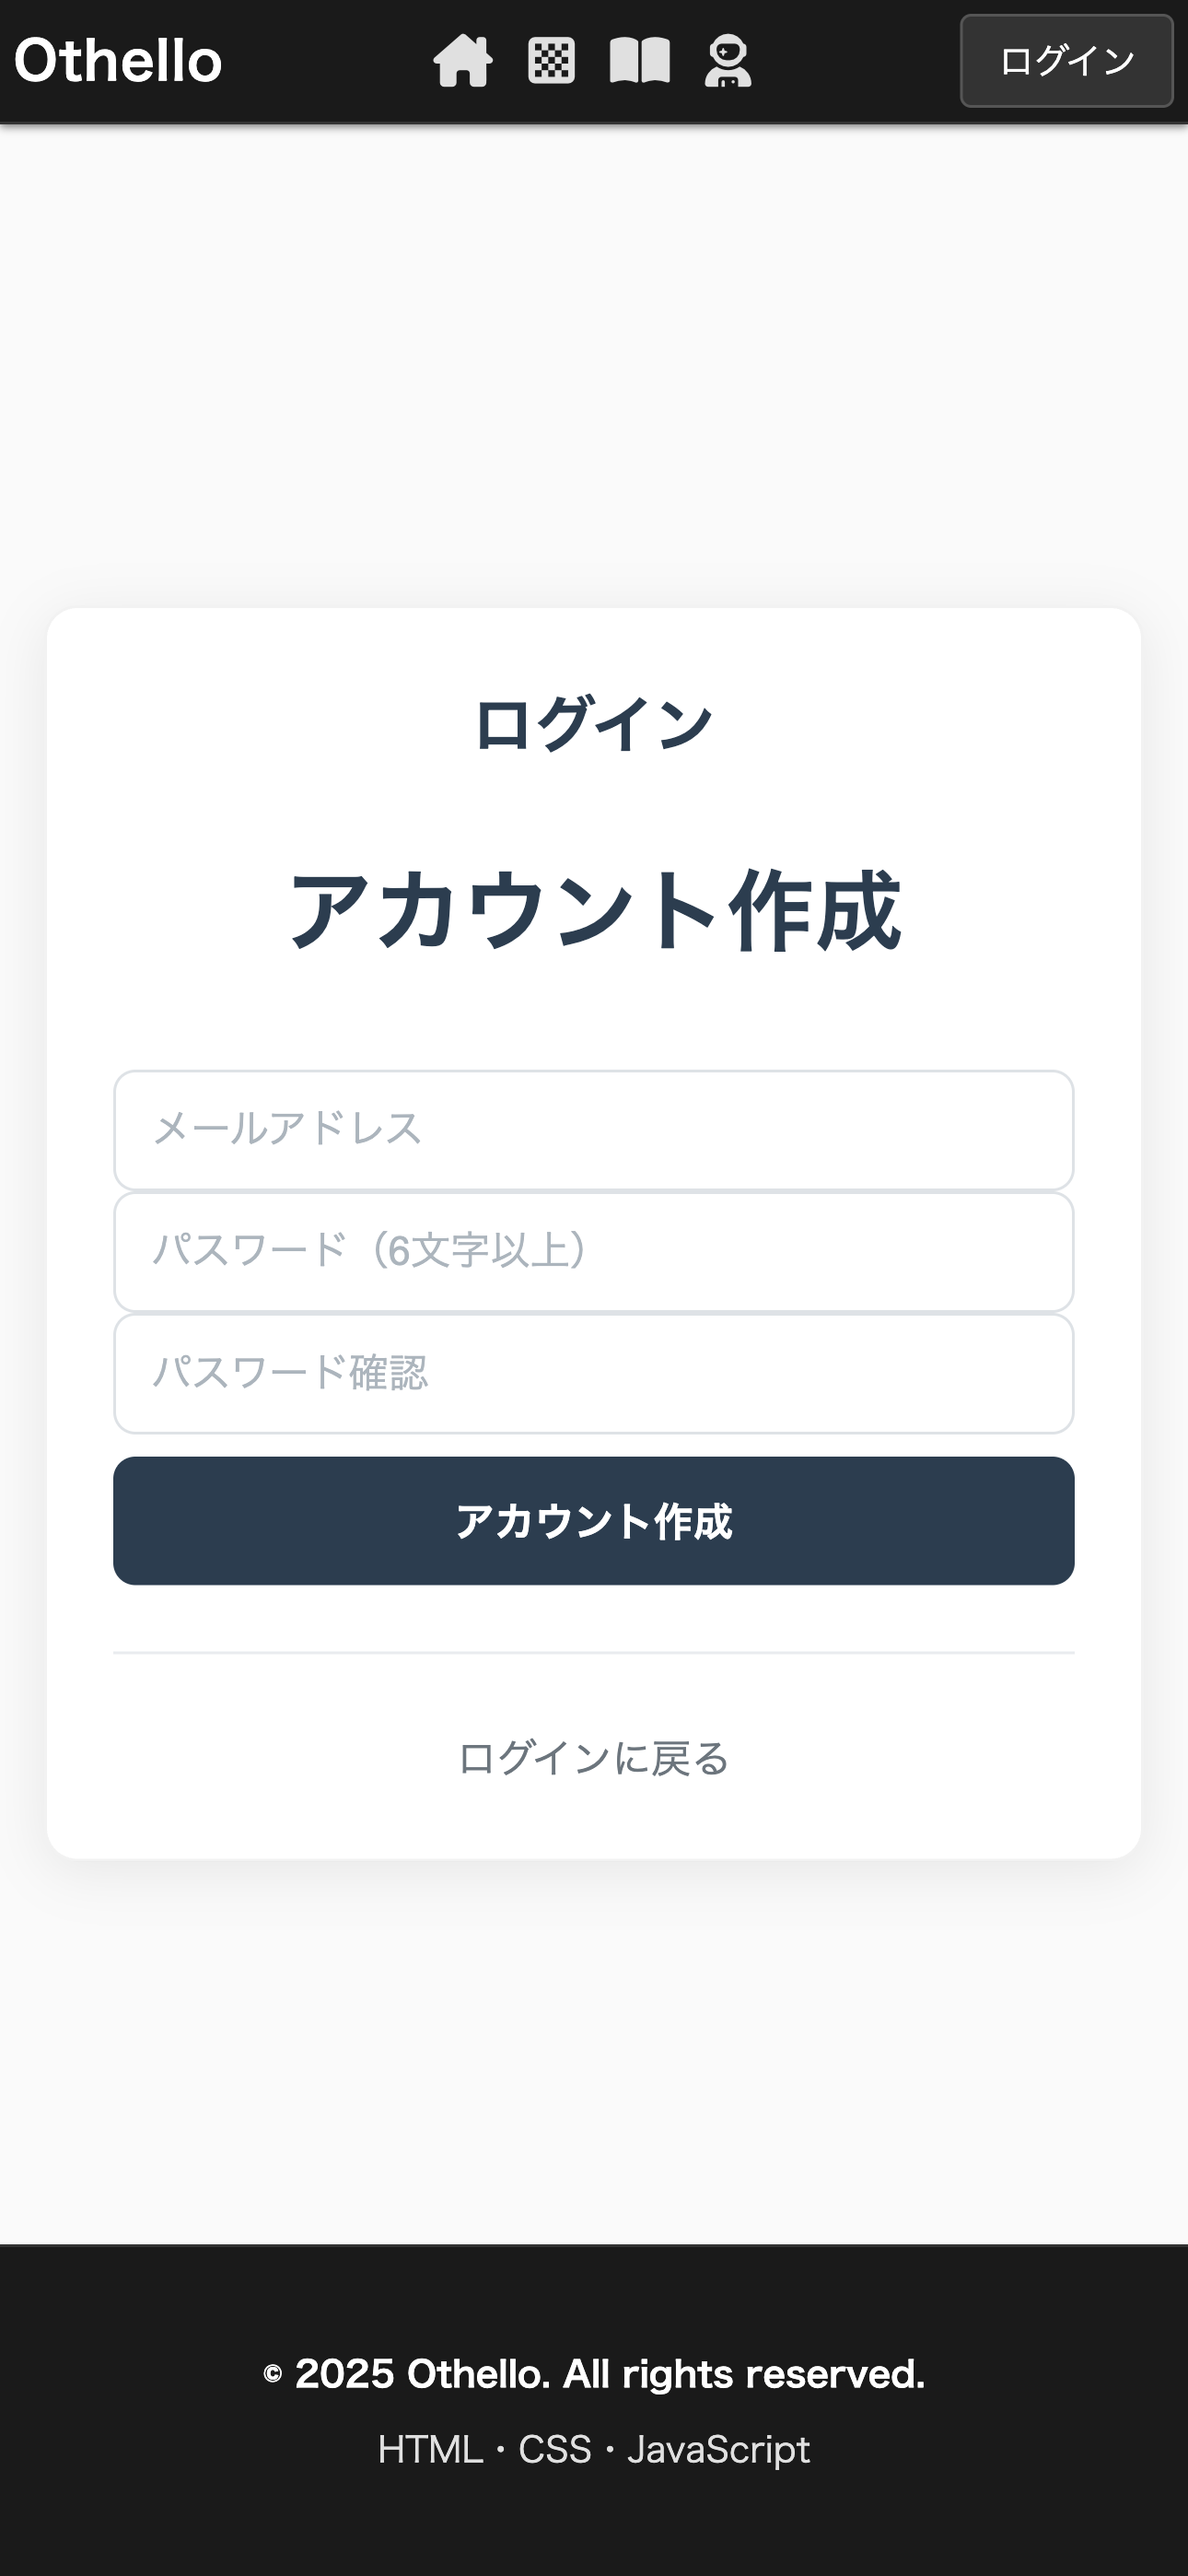
\includegraphics[width=0.4\textwidth]{img/signup-phone.png}
\caption{サインアップ画面(スマートフォン版)}
\label{fig:signup-phone}
\end{figure}

\subsection{認証メール}
図\ref{fig:mail-from-supabase}に実際に届いた認証メールを示す.

\begin{figure}[H]
\centering
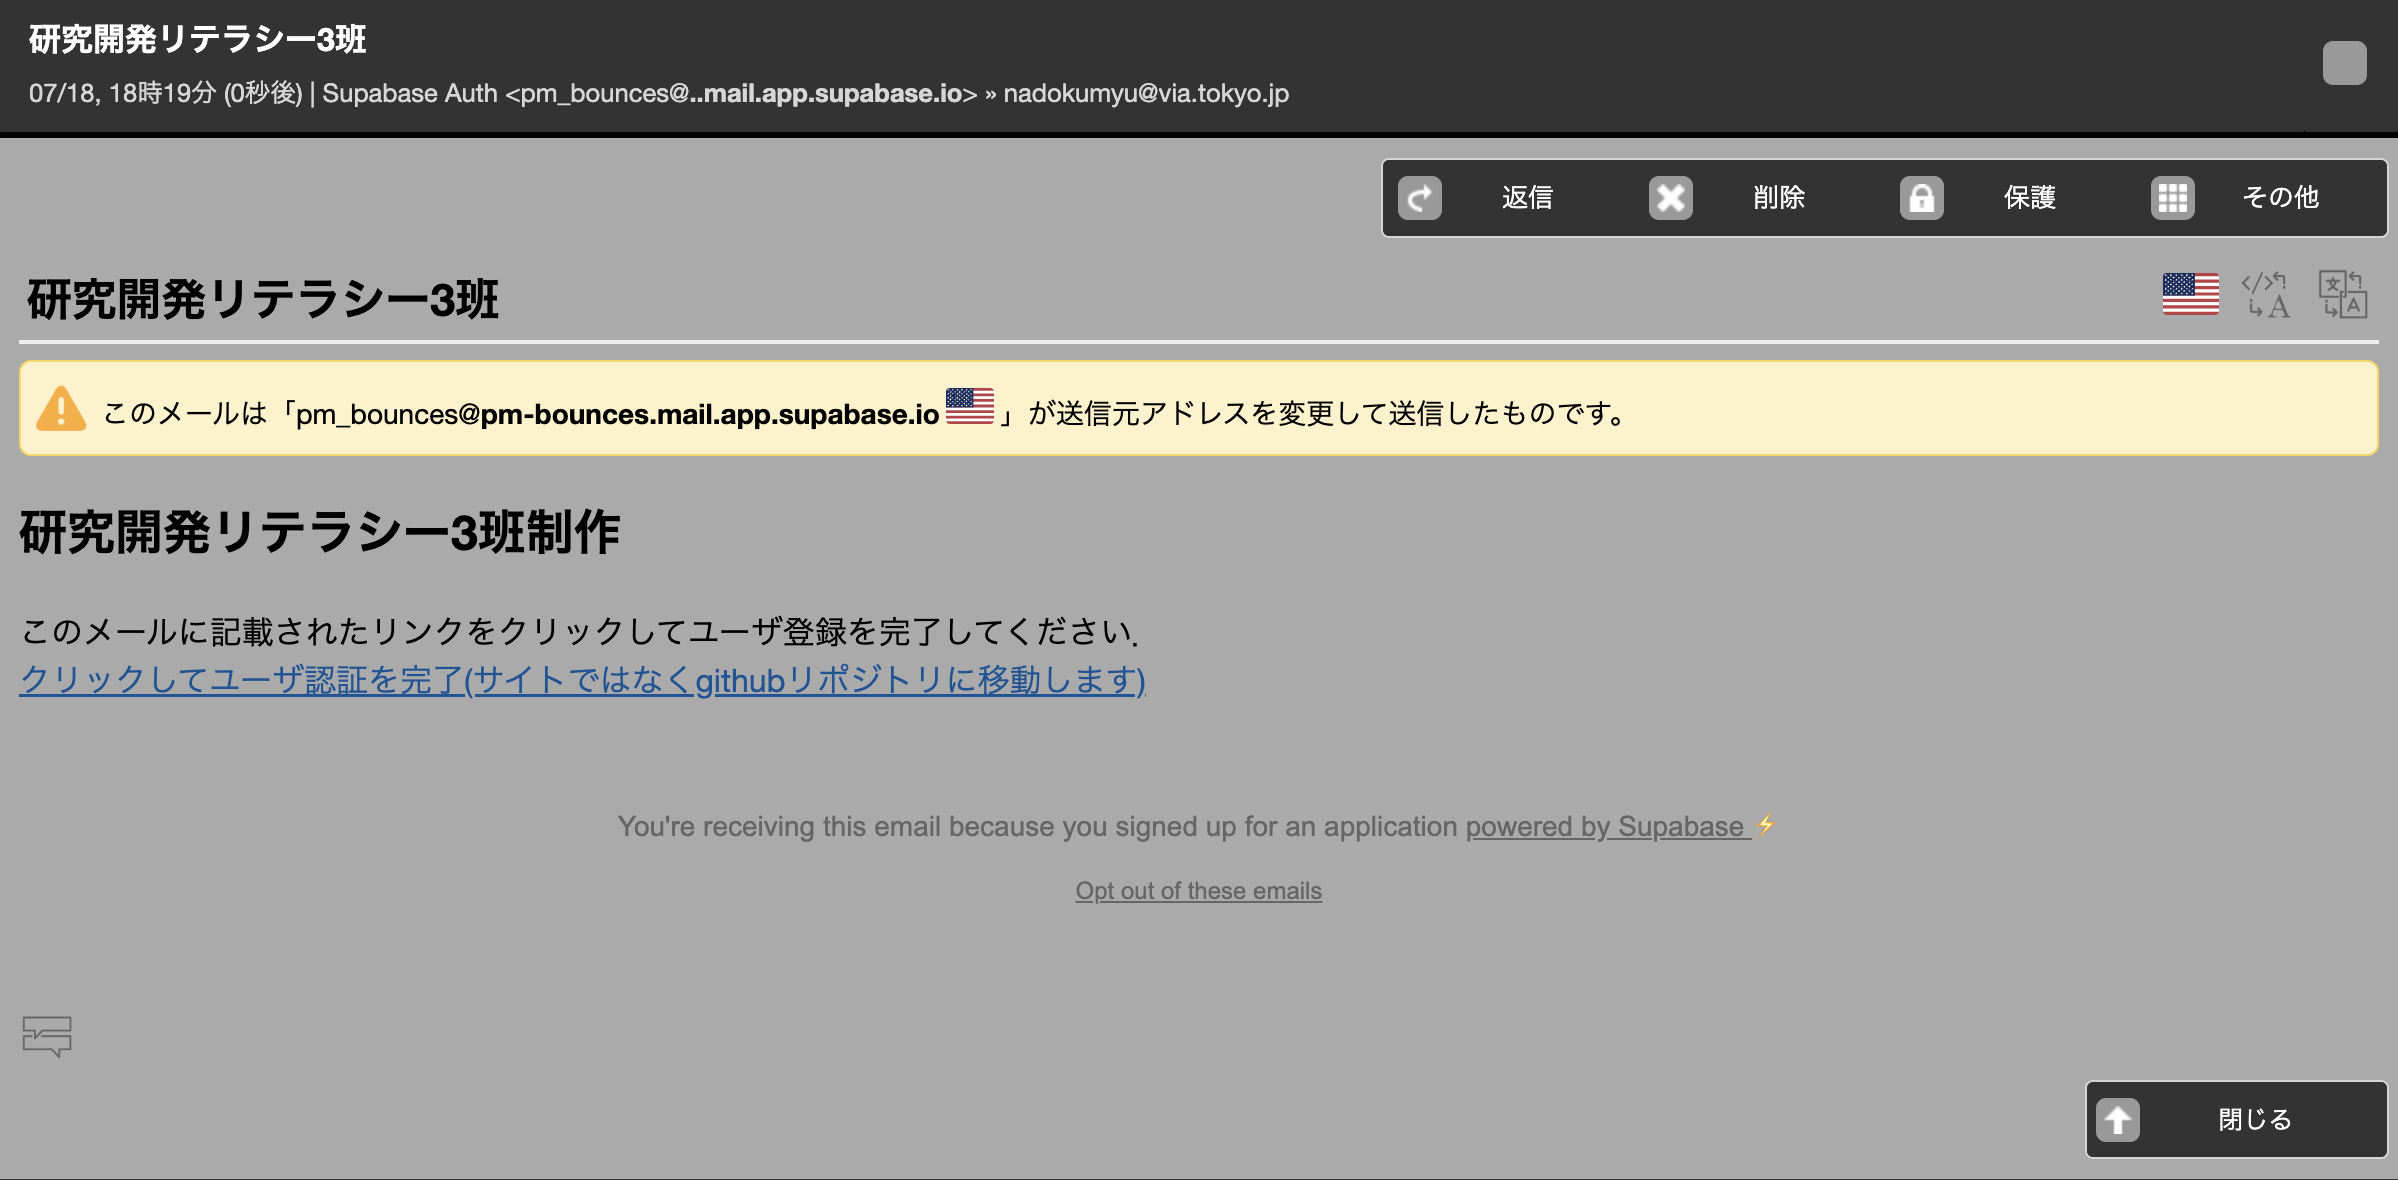
\includegraphics[width=0.7\textwidth]{img/mail-from-supabase.png}
\caption{Supabaseから届いた認証メール}
\label{fig:mail-from-supabase}
\end{figure}

\subsection{ログイン済み画面}
図\ref{fig:loggedin-pc}と図\ref{fig:loggedin-phone}にログイン済みの状態を示す.

\begin{figure}[H]
\centering
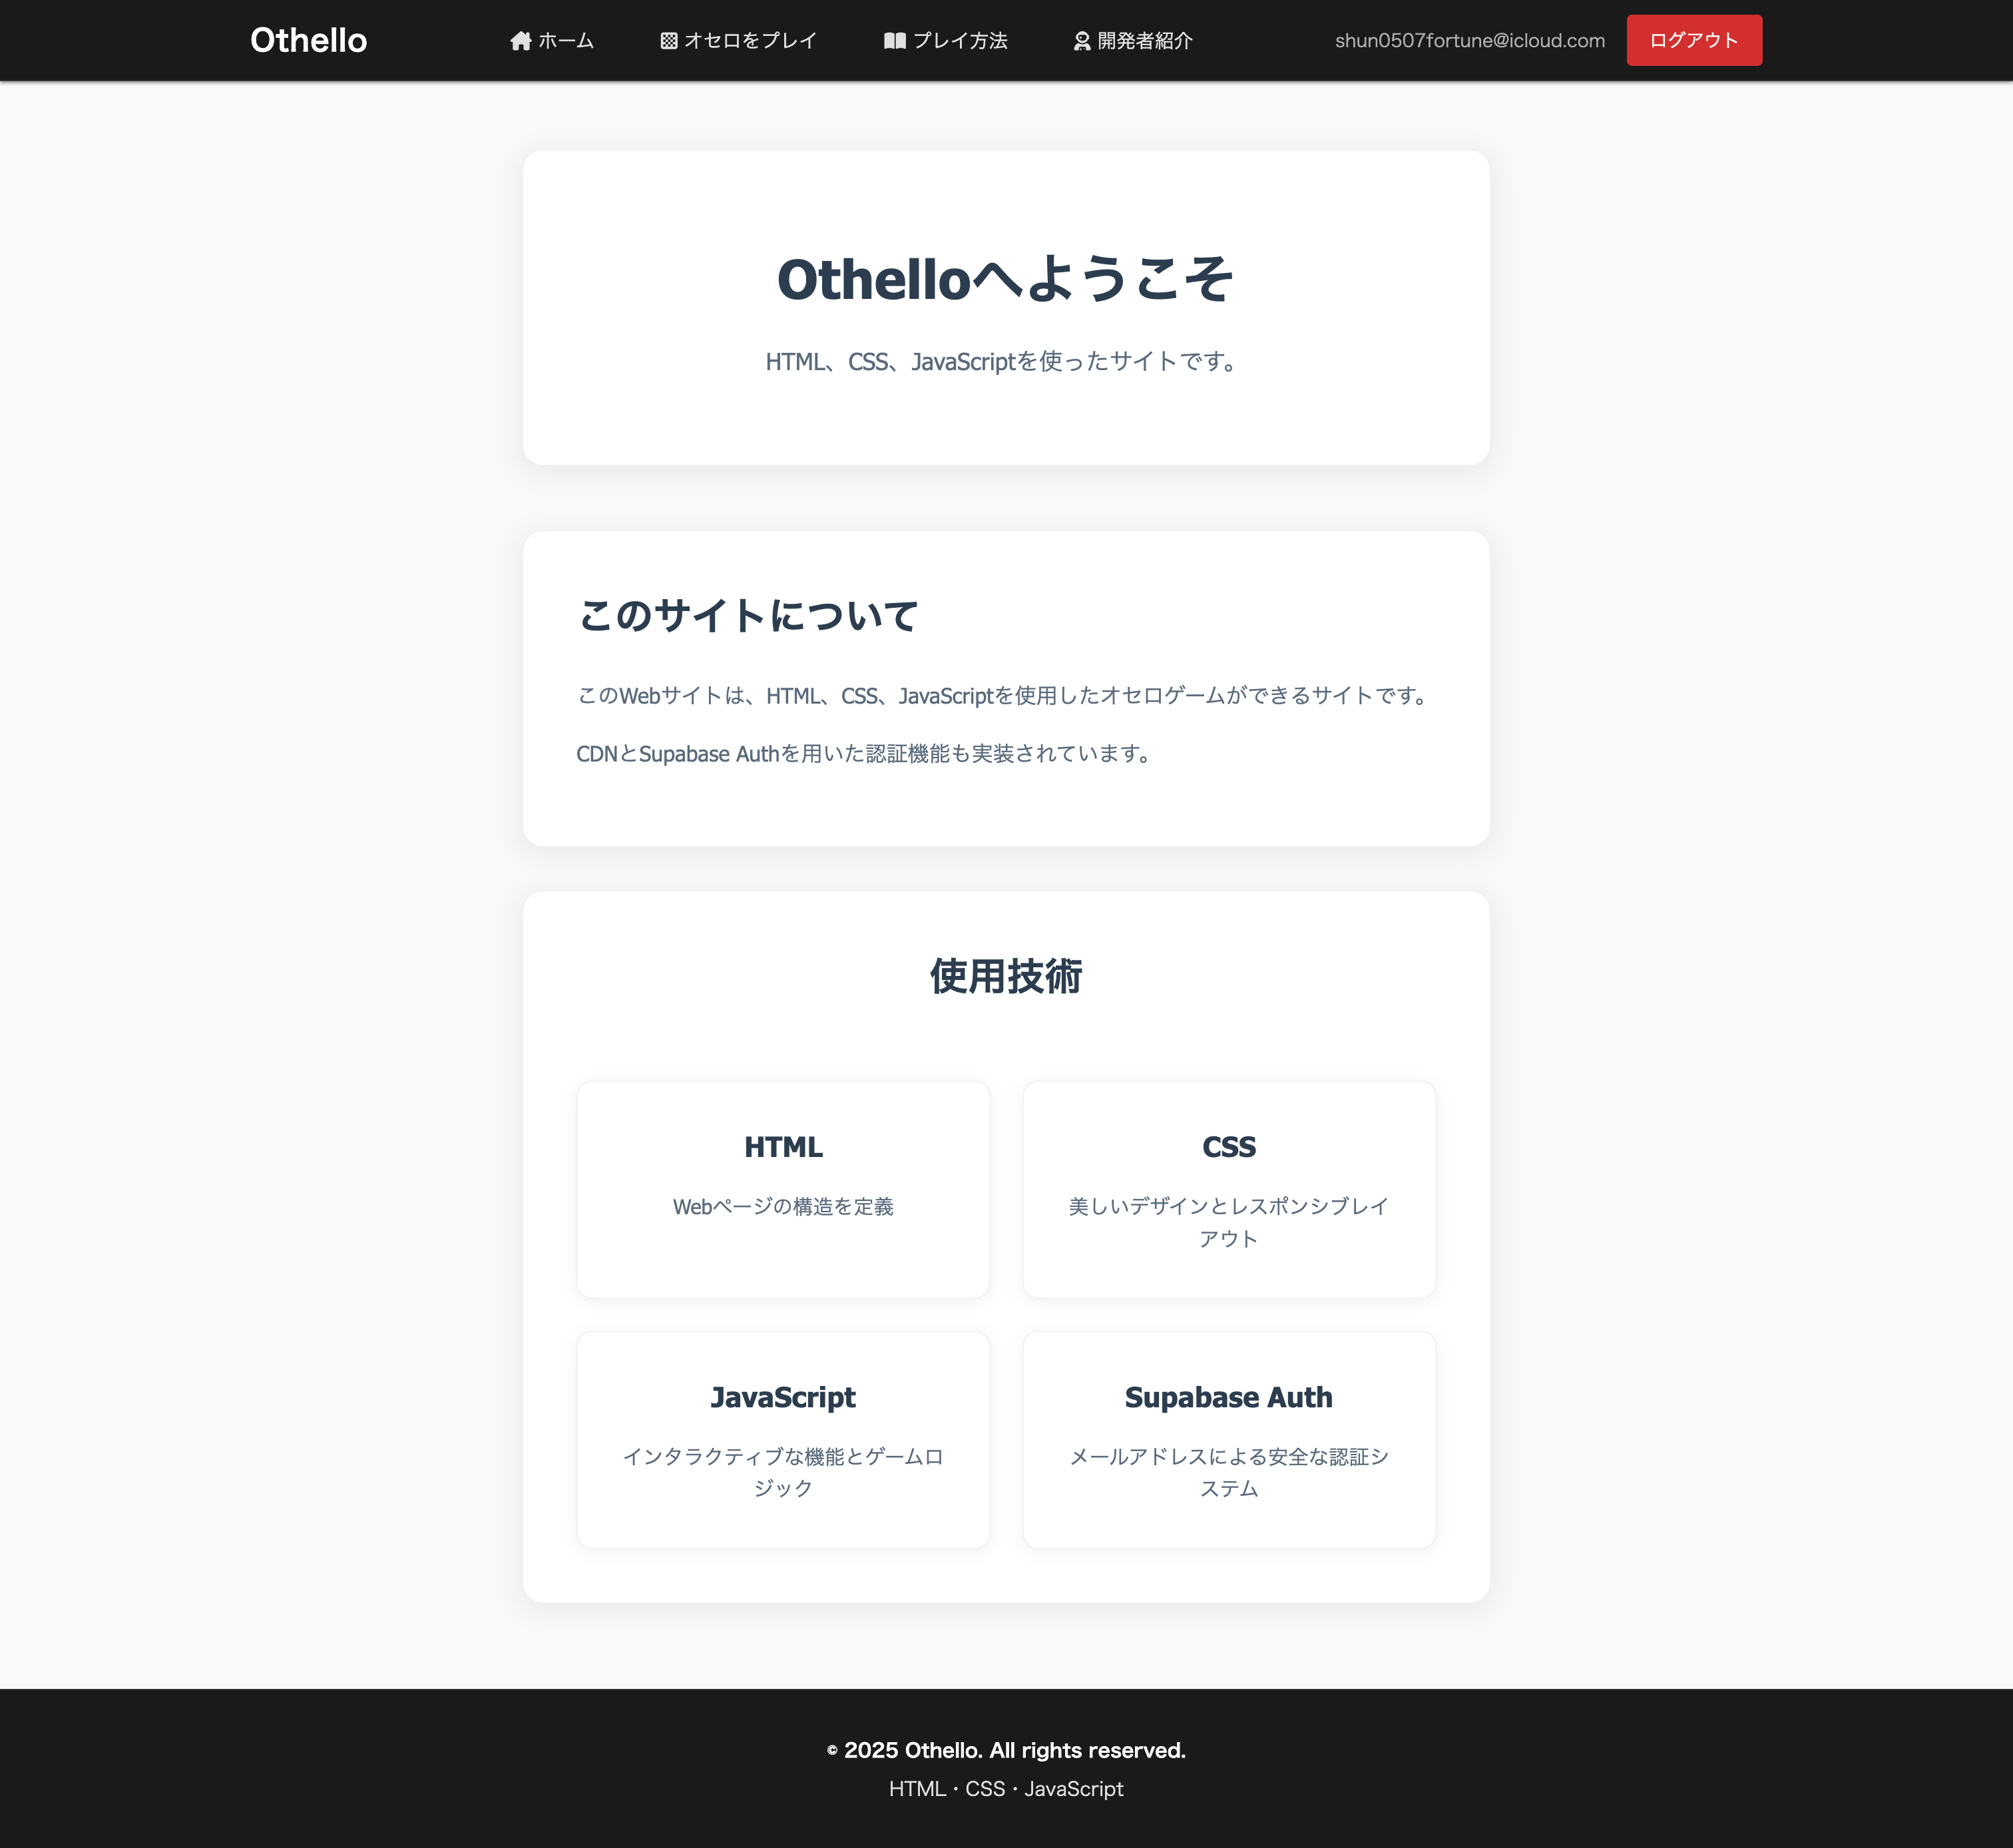
\includegraphics[width=0.7\textwidth]{img/loggedin-pc.png}
\caption{ログイン済み画面(PC版)}
\label{fig:loggedin-pc}
\end{figure}

\begin{figure}[H]
\centering
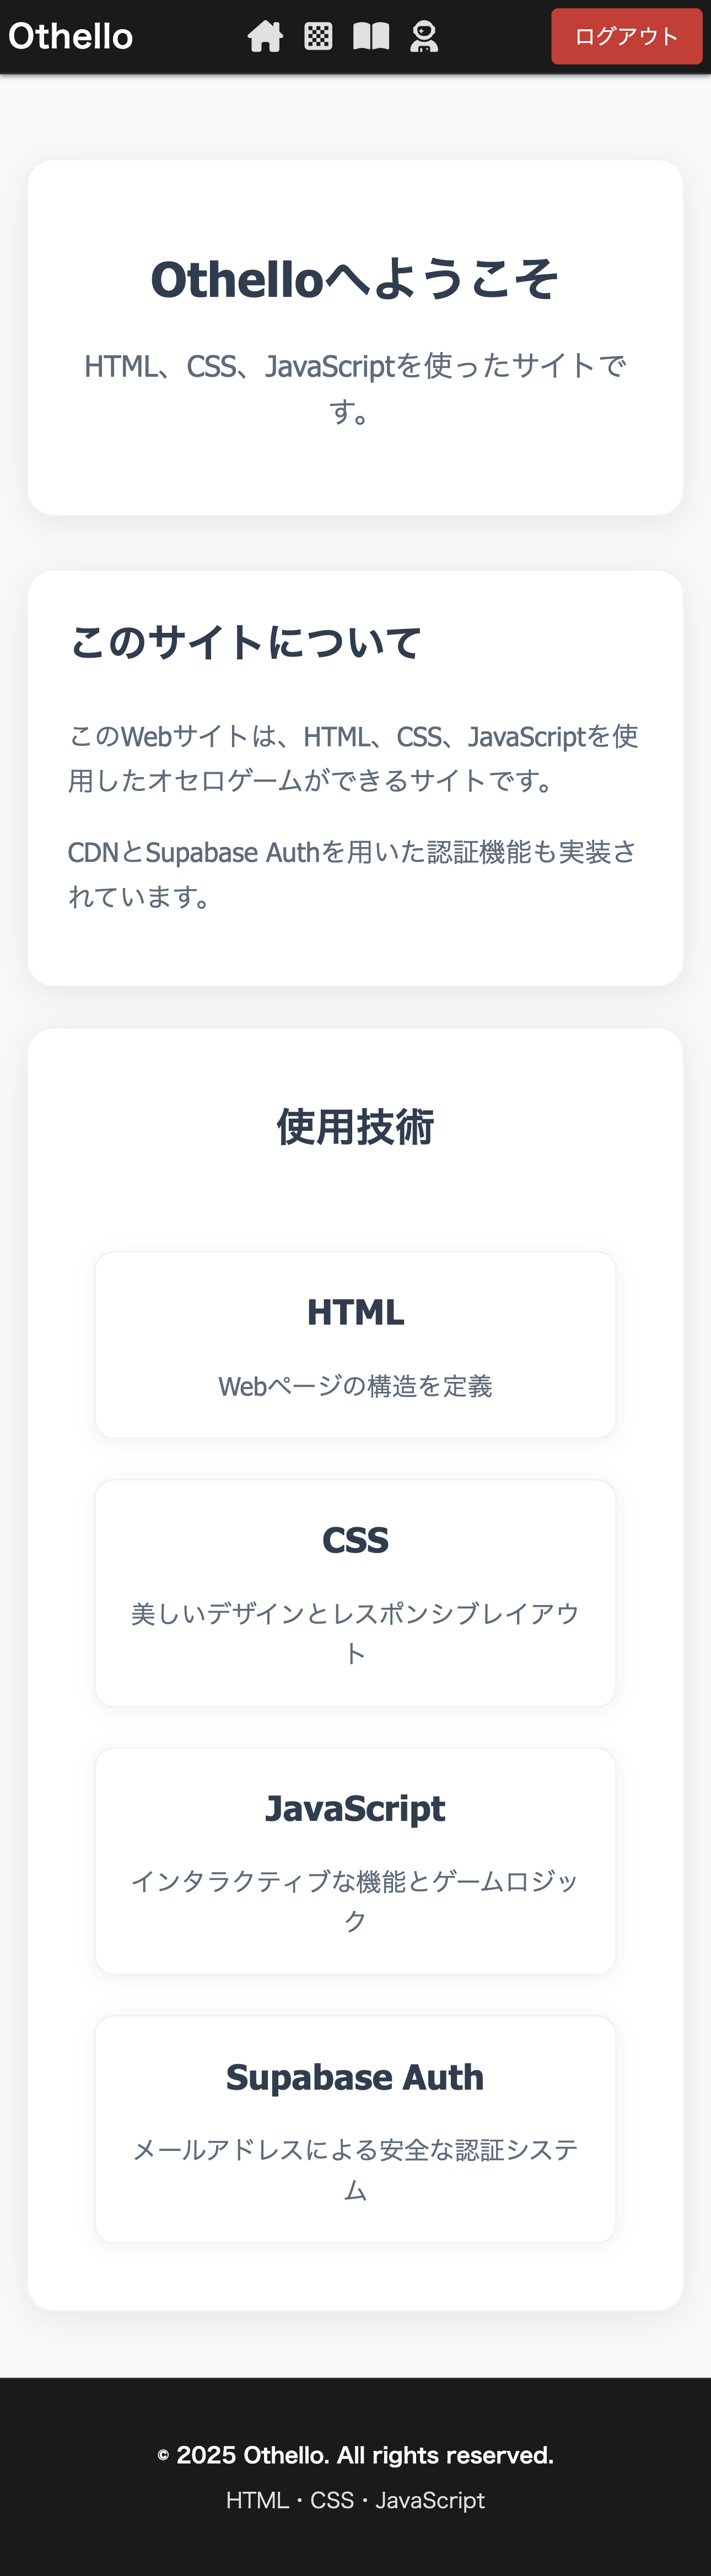
\includegraphics[width=0.4\textwidth]{img/loggedin-phone.png}
\caption{ログイン済み画面(スマートフォン版)}
\label{fig:loggedin-phone}
\end{figure}

\subsection{遊び方説明ページ}
図\ref{fig:howto-pc}と図\ref{fig:howto-phone}に遊び方説明ページを示す.

\begin{figure}[H]
\centering
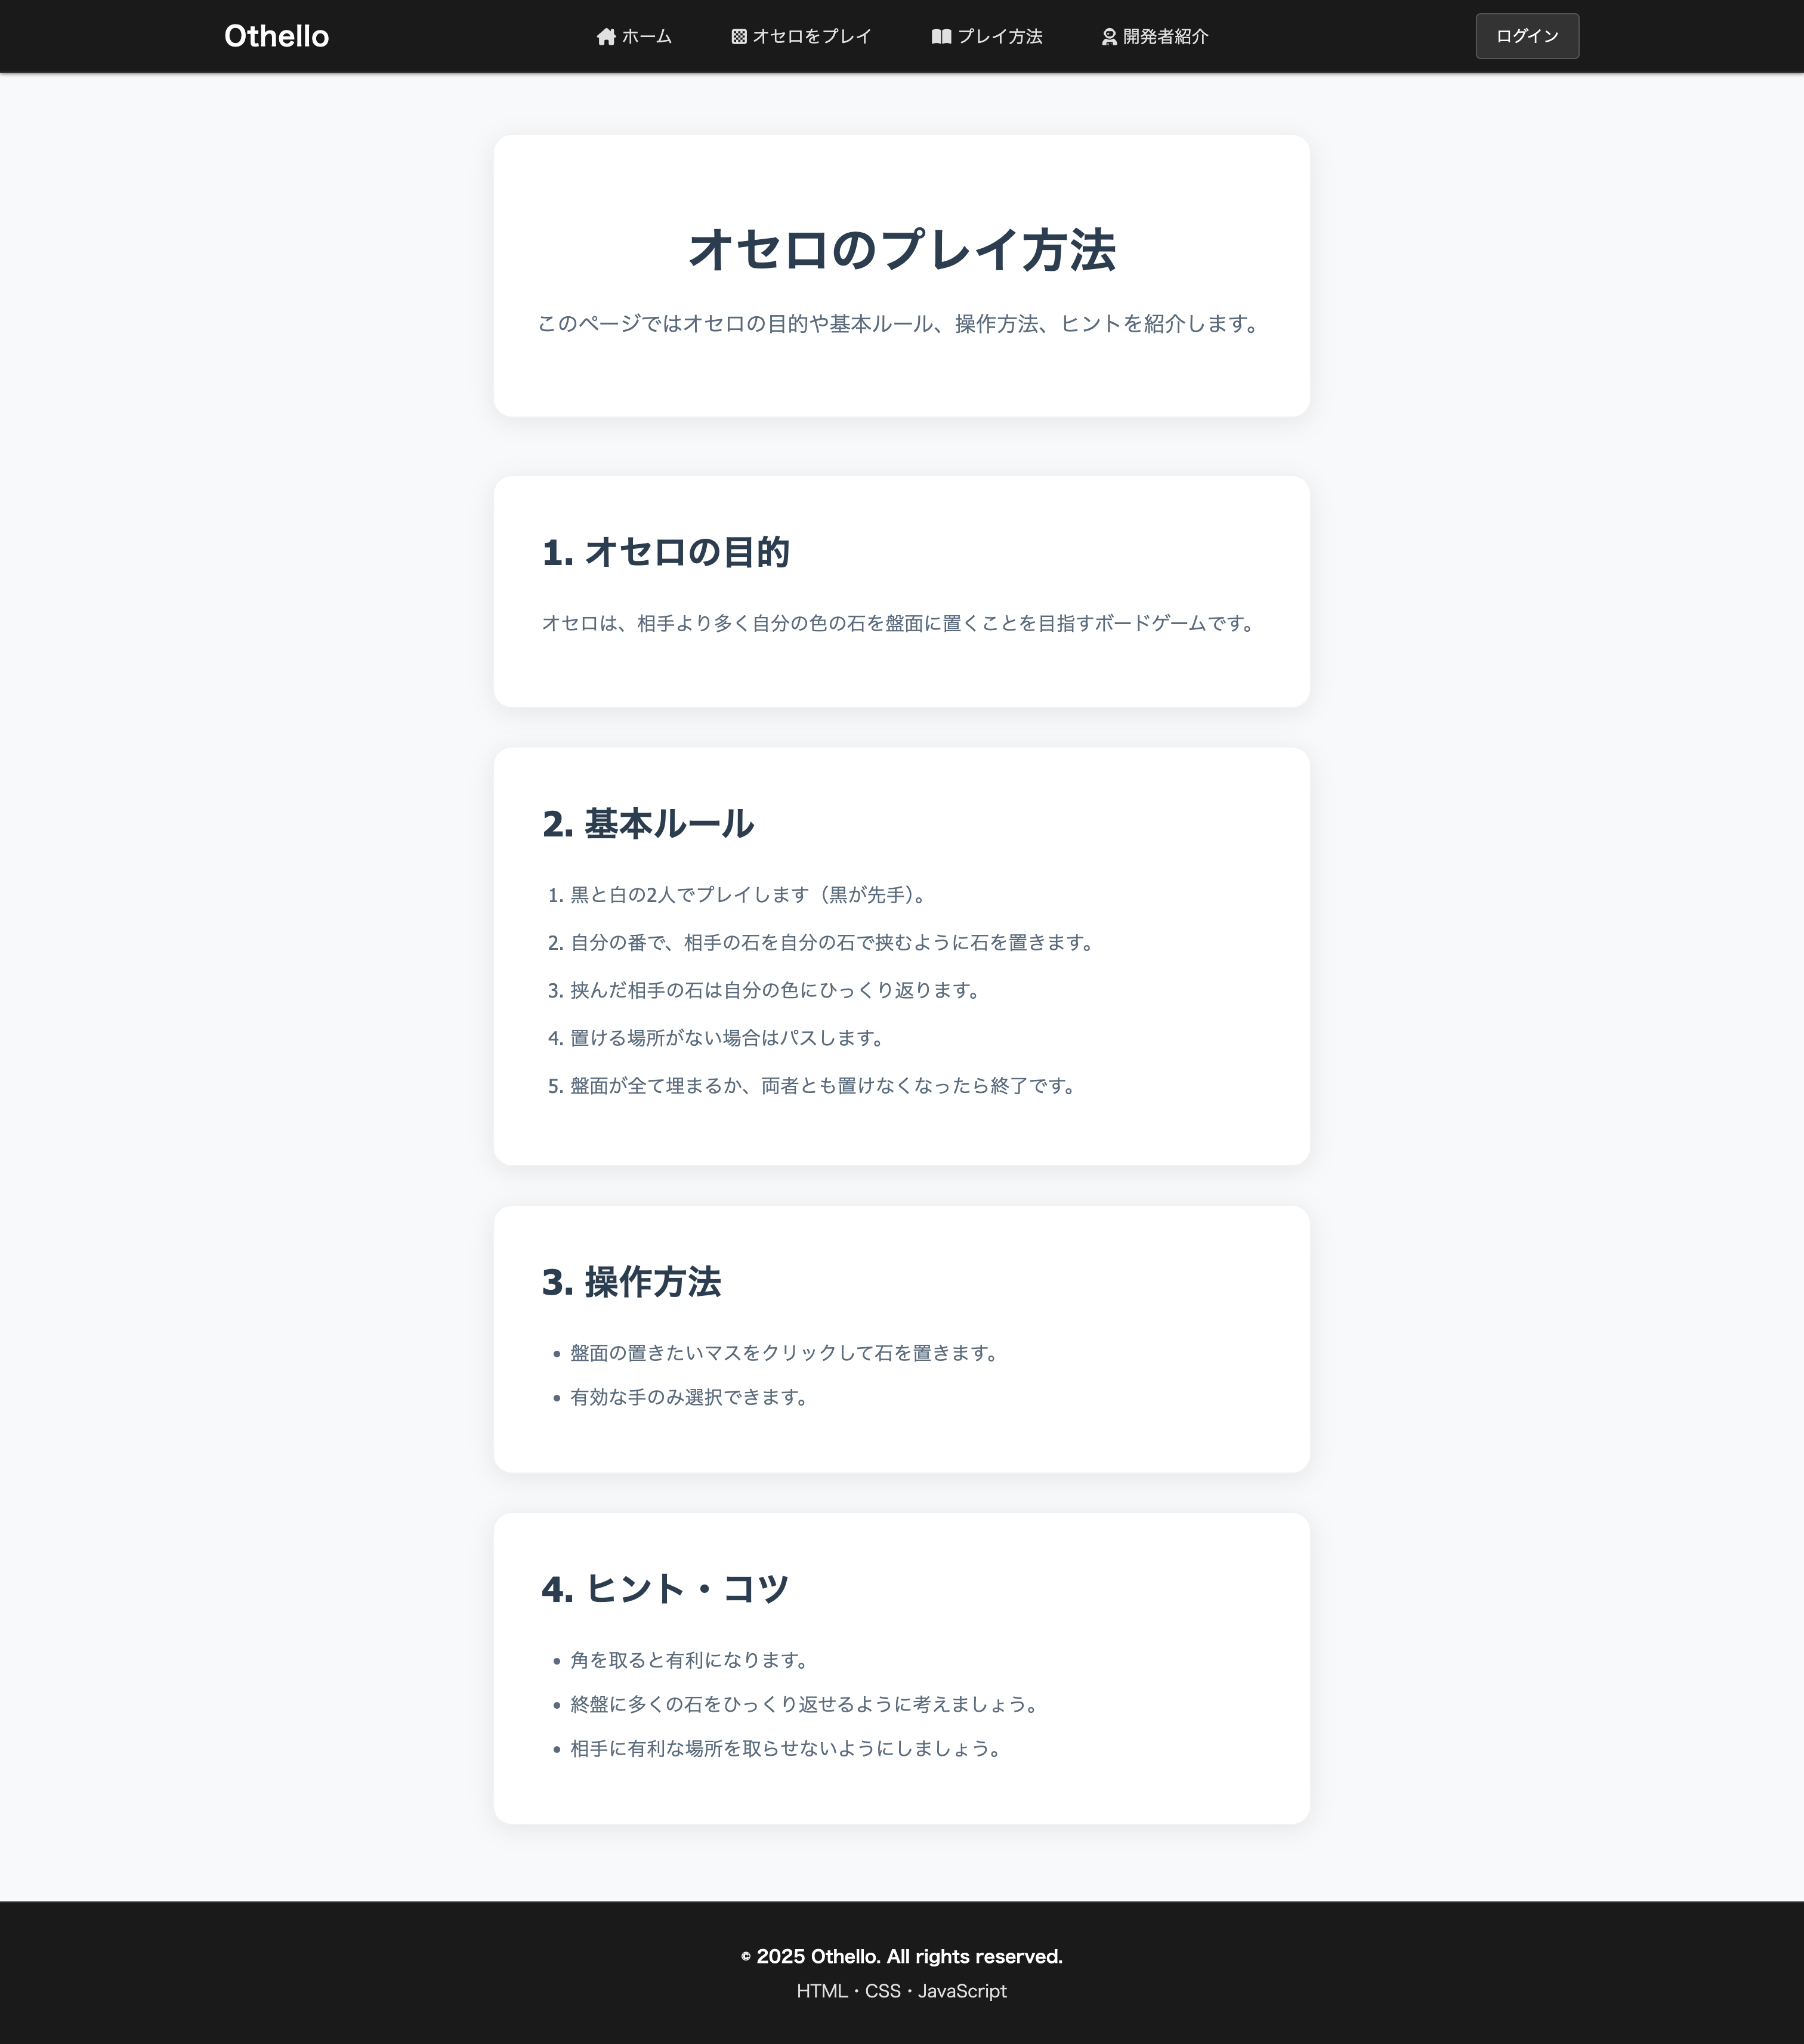
\includegraphics[width=0.7\textwidth]{img/howto-pc.png}
\caption{遊び方説明ページ(PC版)}
\label{fig:howto-pc}
\end{figure}

\begin{figure}[H]
\centering
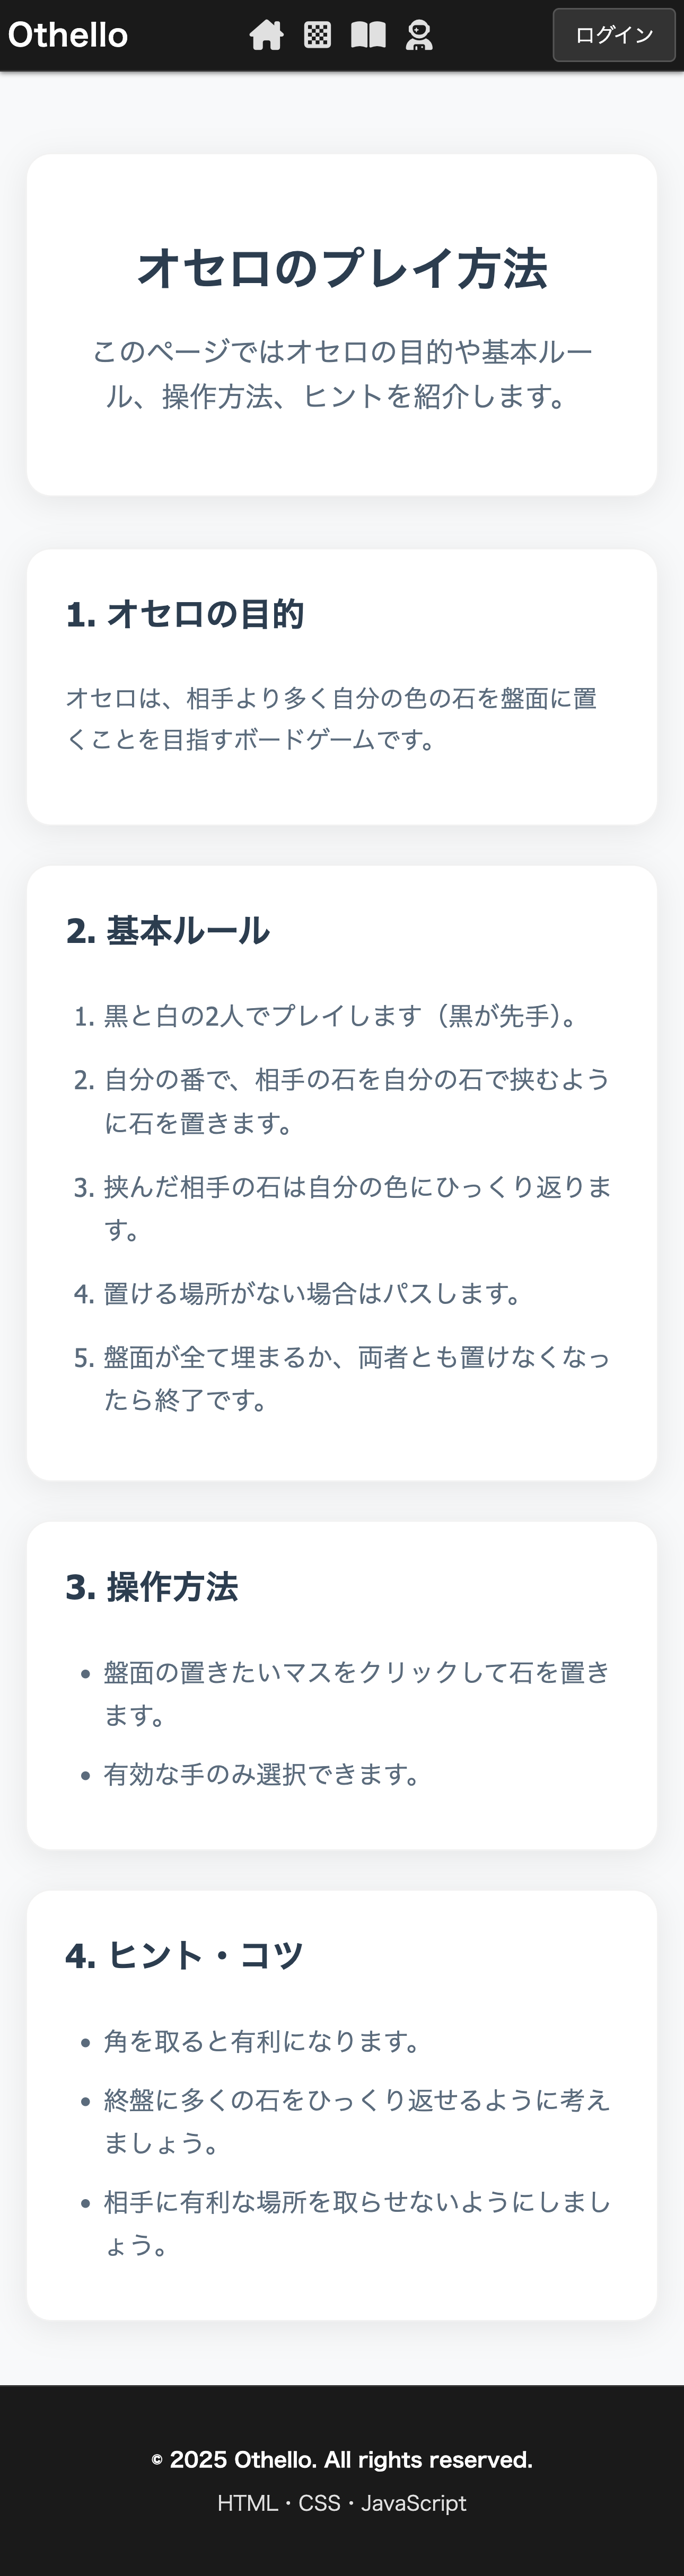
\includegraphics[width=0.4\textwidth]{img/howto-phone.png}
\caption{遊び方説明ページ(スマートフォン版)}
\label{fig:howto-phone}
\end{figure}

\subsection{開発者紹介ページ}
図\ref{fig:developer-pc}と図\ref{fig:developer-phone}に開発者紹介ページを示す.

\begin{figure}[H]
\centering
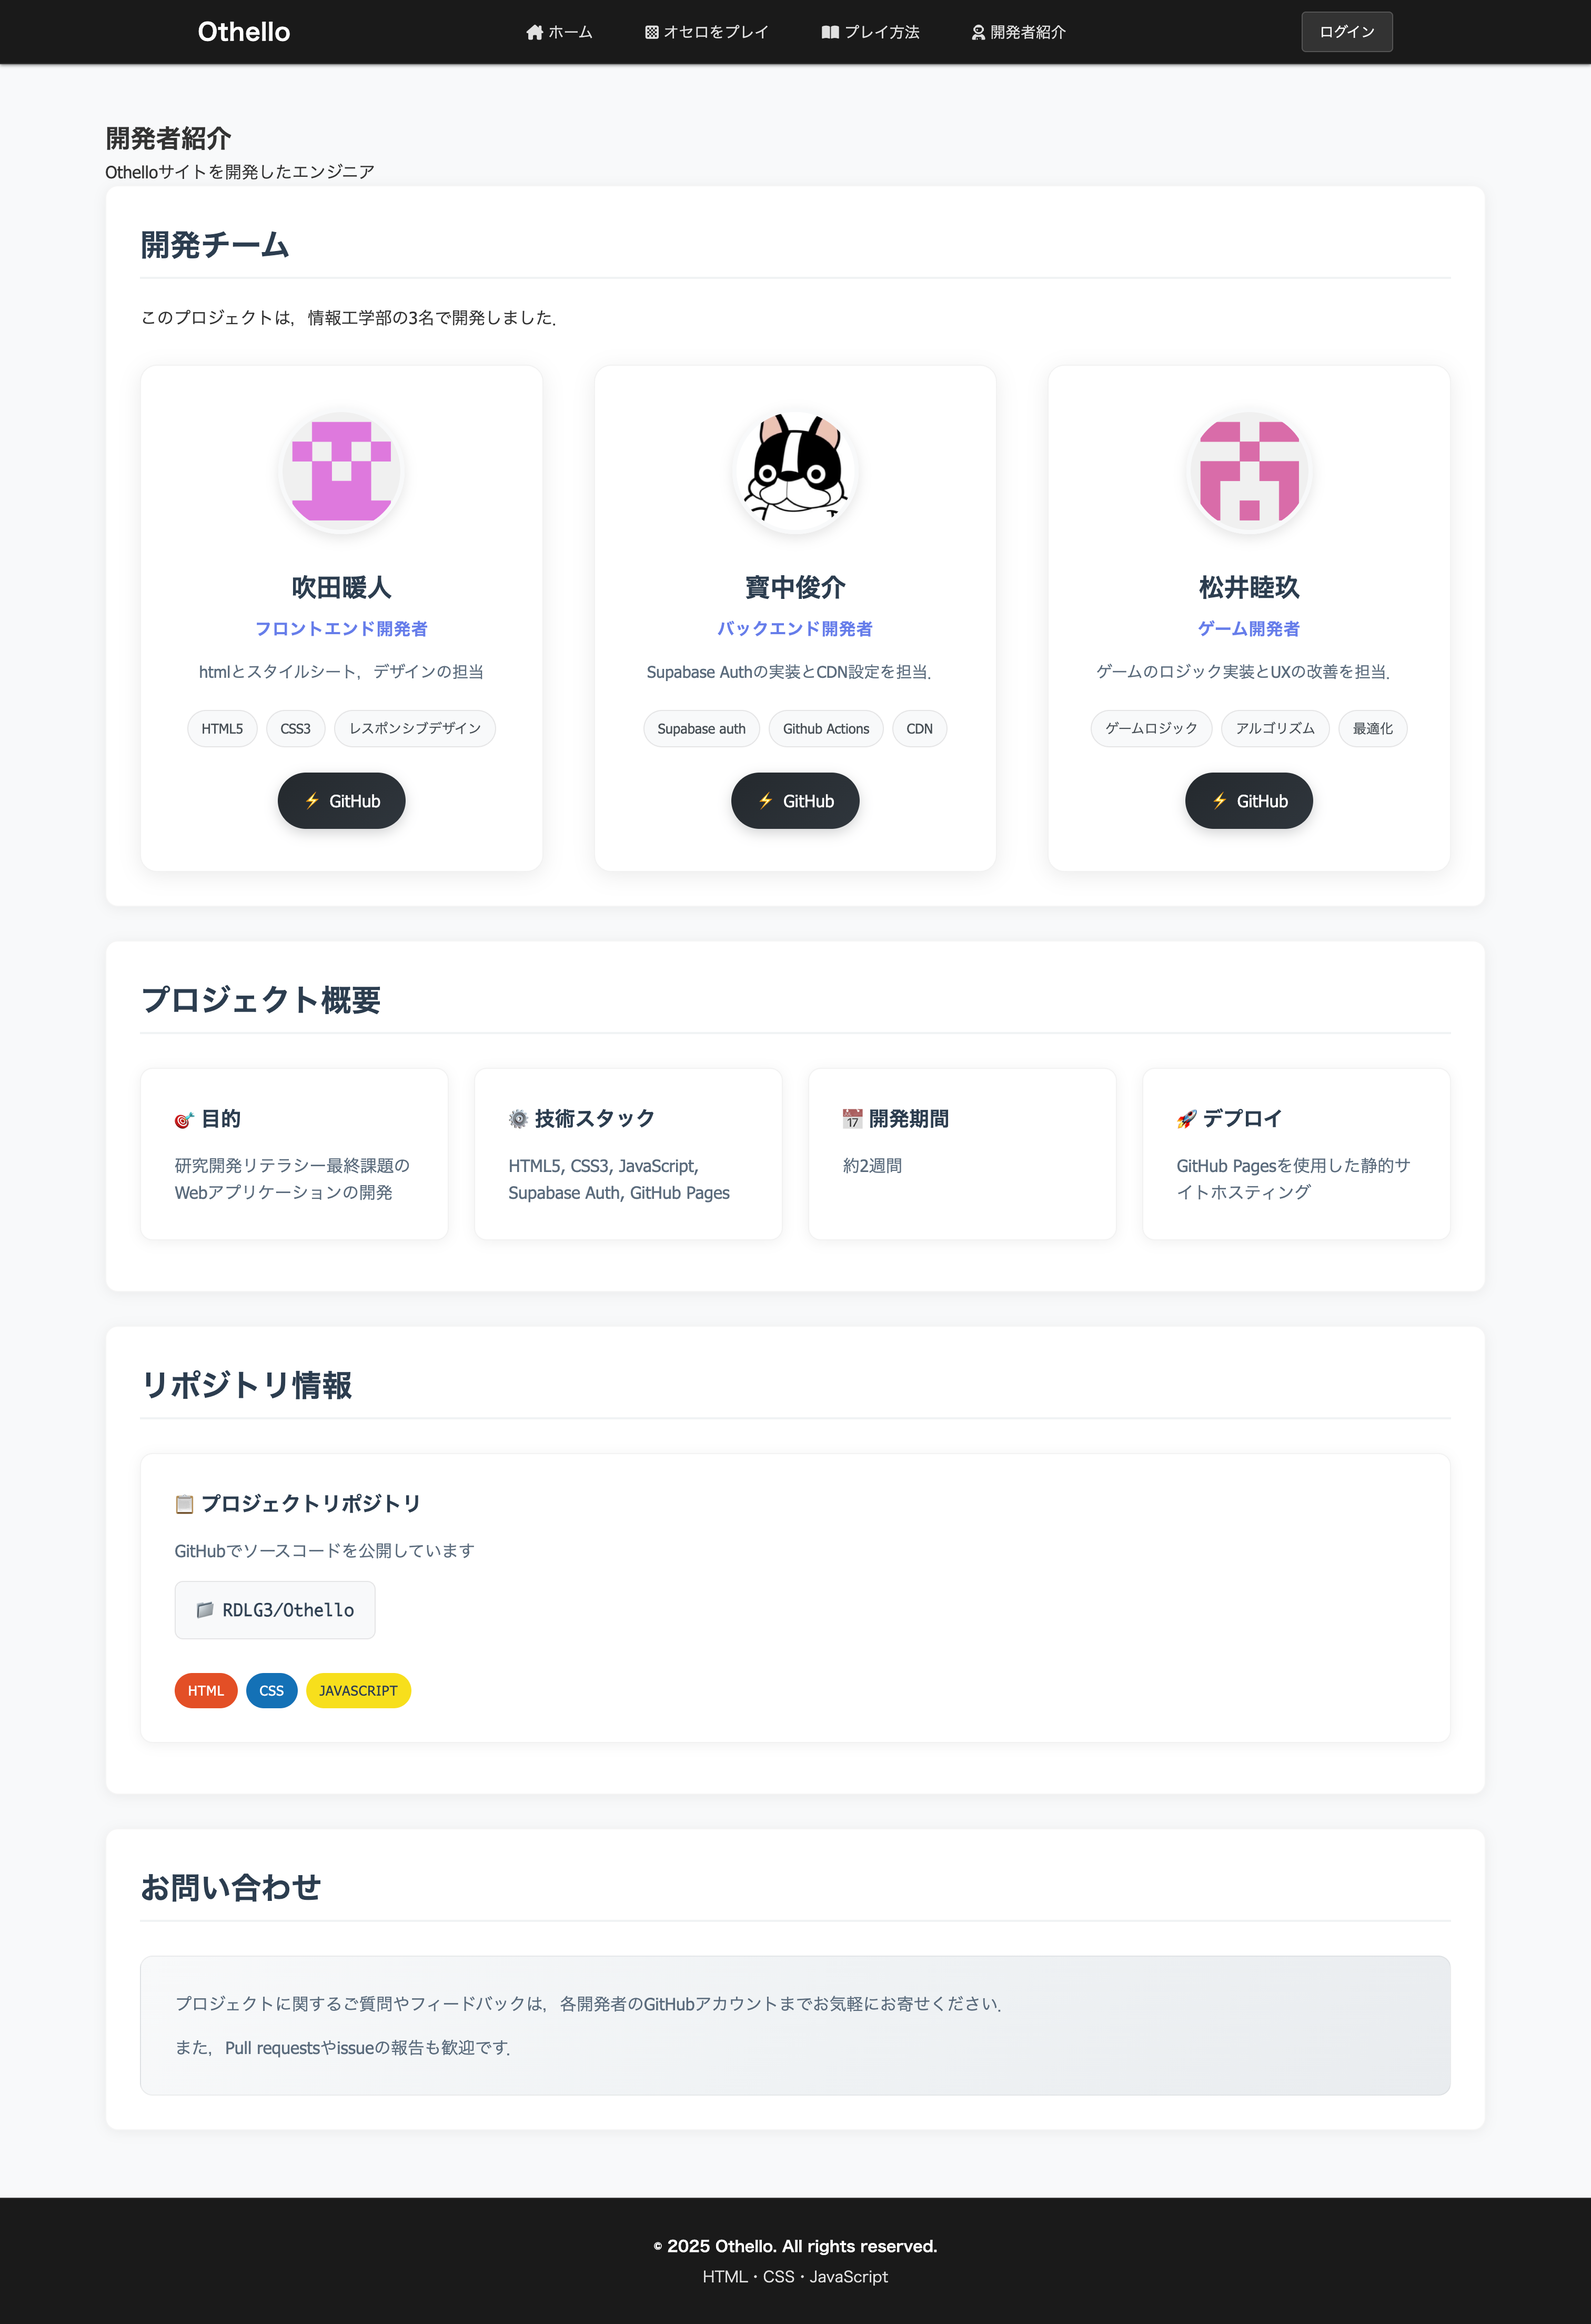
\includegraphics[width=0.7\textwidth]{img/developer-pc.png}
\caption{開発者紹介ページ(PC版)}
\label{fig:developer-pc}
\end{figure}

\begin{figure}[H]
\centering

\includegraphics[width=0.4\textwidth]{img/developer-phone.png}
\caption{開発者紹介ページ(スマートフォン版)}
\label{fig:developer-phone}
\end{figure}

\section{アピールポイント}

\subsection{技術的な特徴}
\begin{itemize}
    \item レスポンシブデザインによるマルチデバイス対応
    \item Supabase Authを用いた本格的な認証システム
    \item GitHub Pagesを活用した自動デプロイ
    \item モジュール化されたコード構成
\end{itemize}

\subsection{ユーザビリティ}
\begin{itemize}
    \item 直感的で分かりやすいゲームインターフェース
    \item シンプルで美しいデザイン
    \item 高速な動作とスムーズな操作感
\end{itemize}

\section{まとめ}

本プロジェクトでは,Web技術の実践的な学習とチーム開発の経験を通じて,以下の成果を得ることができた:

\begin{enumerate}
    \item HTML5・CSS3・JavaScriptの実装スキル向上
    \item Git/GitHubを用いた分散開発手法の習得
    \item 外部サービス(Supabase)との連携経験
    \item レスポンシブWebデザインの実装技術
    \item プロジェクト管理とチーム協働の重要性の理解
\end{enumerate}

今後は,ユーザビリティテストの実施やパフォーマンス最適化,新機能の追加などを通じて,さらなる品質向上を目指したい.

本プロジェクトの成果物は以下のURLで公開している:
\url{https://rdlg3.github.io/Othello/}

\end{document}
